% ============================================================
%  Manual de Usuario — Laboratorio de Programación Virtual
%  para el Diseño Lógico Digital mediante Lógica Reconfigurable
% ============================================================
\documentclass[12pt, a4paper, twoside]{book}

% ── Codificación y lenguaje ─────────────────────────────────
\usepackage[utf8]{inputenc}
\usepackage[T1]{fontenc}
\usepackage[spanish]{babel}

% ── Tipografía elegante ─────────────────────────────────────
\usepackage{lmodern}
\usepackage{microtype}

% ── Geometría de página ─────────────────────────────────────
\usepackage[
  top=3cm, bottom=3cm,
  inner=3.5cm, outer=2.5cm,
  headheight=15pt
]{geometry}

% ── Color y gráficos ────────────────────────────────────────
\usepackage[dvipsnames, table]{xcolor}
\usepackage{graphicx}
\usepackage{tikz}
\usepackage{pgfplots}
\pgfplotsset{compat=1.18}

% Paleta principal
\definecolor{PrimaryBlue}{RGB}{0, 61, 124}
\definecolor{AccentBlue}{RGB}{0, 120, 215}
\definecolor{LightGray}{RGB}{245, 247, 250}
\definecolor{DarkGray}{RGB}{60, 60, 60}
\definecolor{SuccessGreen}{RGB}{34, 139, 34}
\definecolor{WarnOrange}{RGB}{204, 102, 0}

% ── Encabezados y pies de página ────────────────────────────
\usepackage{fancyhdr}
\pagestyle{fancy}
\fancyhf{}
\fancyhead[LE]{\small\color{PrimaryBlue}\leftmark}
\fancyhead[RO]{\small\color{PrimaryBlue}\rightmark}
\fancyfoot[C]{\small\color{DarkGray}\thepage}
\renewcommand{\headrulewidth}{0.4pt}
\renewcommand{\headrule}{\color{AccentBlue}\hrule width\headwidth height\headrulewidth}

% ── Capítulos y secciones (titlesec) ────────────────────────
\usepackage{titlesec}
\usepackage{titletoc}

\titleformat{\chapter}[display]
  {\normalfont}
  {\raggedleft\fontsize{72}{72}\selectfont\color{DarkGray!18}\thechapter}
  {-14pt}
  {\huge\bfseries\color{DarkGray}}
  [{\vspace{6pt}\color{AccentBlue}\titlerule[1pt]}]
\titlespacing*{\chapter}{0pt}{20pt}{32pt}

\titleformat{\section}
  {\normalfont\Large\bfseries\color{DarkGray}}
  {\thesection}{1em}{}
  [{\vspace{2pt}\color{DarkGray!30}\titlerule[0.5pt]}]

\titleformat{\subsection}
  {\normalfont\large\bfseries\color{DarkGray}}
  {\thesubsection}{1em}{}

\titleformat{\subsubsection}
  {\normalfont\normalsize\bfseries\itshape\color{DarkGray}}
  {\thesubsubsection}{1em}{}

% ── Listas y enumeraciones ──────────────────────────────────
\usepackage{enumitem}
\setlist[itemize,1]{label=\textcolor{AccentBlue}{\textbullet}}
\setlist[itemize,2]{label=\textcolor{PrimaryBlue}{\textendash}}

% ── Cajas y avisos ──────────────────────────────────────────
\usepackage[most]{tcolorbox}

\tcbset{
  base style/.style={
    enhanced, arc=4pt, boxrule=0pt,
    left=6pt, right=6pt, top=6pt, bottom=6pt,
    fonttitle=\bfseries\small,
  }
}

\newtcolorbox{notebox}[1][Nota]{
  base style,
  colback=AccentBlue!10, colframe=AccentBlue,
  title={#1}, attach boxed title to top left={xshift=8pt, yshift=-4pt},
  boxed title style={colback=AccentBlue, arc=3pt, boxrule=0pt}
}

\newtcolorbox{warnbox}[1][Advertencia]{
  base style,
  colback=WarnOrange!10, colframe=WarnOrange,
  title={#1}, attach boxed title to top left={xshift=8pt, yshift=-4pt},
  boxed title style={colback=WarnOrange, arc=3pt, boxrule=0pt}
}

\newtcolorbox{tipbox}[1][Consejo]{
  base style,
  colback=SuccessGreen!8, colframe=SuccessGreen,
  title={#1}, attach boxed title to top left={xshift=8pt, yshift=-4pt},
  boxed title style={colback=SuccessGreen, arc=3pt, boxrule=0pt}
}

% Paso numerado (para procedimientos)
\newtcolorbox{stepbox}[1]{
  base style,
  colback=LightGray, colframe=PrimaryBlue, boxrule=1pt,
  title={Paso #1}, fonttitle=\bfseries\color{white},
  attach boxed title to top left={xshift=8pt, yshift=-4pt},
  boxed title style={colback=PrimaryBlue, arc=3pt}
}

% ── Código fuente ───────────────────────────────────────────
\usepackage{listings}
\lstset{
  backgroundcolor=\color{LightGray},
  basicstyle=\ttfamily\small\color{DarkGray},
  keywordstyle=\bfseries\color{PrimaryBlue},
  commentstyle=\itshape\color{SuccessGreen!70!black},
  stringstyle=\color{WarnOrange},
  numberstyle=\tiny\color{DarkGray!60},
  numbers=left, numbersep=8pt,
  breaklines=true, keepspaces=true,
  frame=single, framerule=0.4pt, rulecolor=\color{AccentBlue!40},
  xleftmargin=15pt, xrightmargin=5pt,
  captionpos=b,
  showstringspaces=false,
}

% Lenguaje VHDL básico
\lstdefinelanguage{VHDL}{
  morekeywords={
    entity, architecture, port, in, out, inout, buffer, signal,
    process, begin, end, if, then, else, elsif, case, when,
    std_logic, std_logic_vector, integer, boolean,
    library, use, all, is, of, downto, to, others,
    component, map, generic, wait, rising_edge, falling_edge
  },
  morecomment=[l]{--},
  morestring=[b]{"},
  sensitive=false
}

% ── Hipervínculos ───────────────────────────────────────────
\usepackage[
  colorlinks=true,
  linkcolor=PrimaryBlue,
  urlcolor=AccentBlue,
  citecolor=DarkGray,
  bookmarks=true,
  bookmarksnumbered=true,
  pdftitle={Manual de Usuario — Laboratorio de Programación Virtual},
  pdfauthor={Treviño Hernández Jonathan; Peñarrieta Villa Jesús},
  pdfsubject={VPL · VHDL · Lógica Digital Reconfigurable}
]{hyperref}

\usepackage{bookmark}

% ── Tablas ──────────────────────────────────────────────────
\usepackage{booktabs}
\usepackage{array}
\usepackage{longtable}
\newcolumntype{L}[1]{>{\raggedright\arraybackslash}p{#1}}
\newcolumntype{C}[1]{>{\centering\arraybackslash}p{#1}}

% ── Misceláneos ─────────────────────────────────────────────
\usepackage{emptypage}
\usepackage{float}
\usepackage{caption}
\captionsetup{font=small, labelfont={bf,color=PrimaryBlue}}

% ============================================================
%  Macros de utilidad
% ============================================================
\newcommand{\vpl}{\textsc{VPL}\xspace}
\newcommand{\vhdl}{\textsc{VHDL}\xspace}
\newcommand{\moodle}{\textit{Moodle}\xspace}
\newcommand{\archivo}[1]{\texttt{\small#1}}
\newcommand{\menu}[1]{\textsf{\textbf{#1}}}

\usepackage{xspace}

% ============================================================
%  DOCUMENTO
% ============================================================
\begin{document}

% ── Portada ─────────────────────────────────────────────────
\begin{titlepage}
  \pagecolor{PrimaryBlue}
  \color{white}
  \centering
  \vspace*{1.5cm}

  % Logo o símbolo decorativo
  \begin{tikzpicture}
    \draw[white, line width=2pt] (0,0) rectangle (3,3);
    \draw[AccentBlue!60, line width=1.2pt] (0.3,0.3) rectangle (2.7,2.7);
    \node[white, font=\Huge\bfseries] at (1.5,1.5) {VPL};
  \end{tikzpicture}

  \vspace{1cm}
  {\fontsize{11}{13}\selectfont\scshape Laboratorio de Programación Virtual}\\[0.4cm]
  {\fontsize{11}{13}\selectfont\scshape para el Diseño Lógico Digital}\\[0.4cm]
  {\fontsize{11}{13}\selectfont\scshape mediante Lógica Reconfigurable}\\[1cm]

  {\color{AccentBlue!60}\rule{0.6\textwidth}{1pt}}\\[0.8cm]

  {\Huge\bfseries Manual de Usuario}\\[0.5cm]

  {\color{AccentBlue!60}\rule{0.6\textwidth}{1pt}}\\[2cm]

  {\large
    Treviño Hernández Jonathan\\[0.3cm]
    Peñarrieta Villa Jesús
  }\\[2.5cm]

  {\small\color{white!70} Versión 1.0 \textendash{} \the\year}

  \vfill
  {\small\color{white!60}
    Escuela Superior de Cómputo\\
    Ingeniería en Sistemas Computacionales
  }
  \vspace{1cm}
\end{titlepage}

\nopagecolor  % restaurar fondo blanco

% ── Página de créditos ──────────────────────────────────────
\thispagestyle{empty}
\vspace*{\fill}
\begin{center}
  \small\color{DarkGray}
  \textbf{Manual de Usuario}\\
  Laboratorio de Programación Virtual para el Diseño Lógico Digital\\
  mediante Lógica Reconfigurable\\[1em]
  \textit{Treviño Hernández Jonathan \textendash{} Peñarrieta Villa Jesús}\\[1em]
  \the\year\\[2em]
  Este documento fue elaborado con fines académicos.\\
  Plataforma: Moodle + Virtual Programming Lab (VPL)
\end{center}
\vspace*{\fill}
\clearpage

% ── Tabla de contenidos ─────────────────────────────────────
\frontmatter
\tableofcontents
\listoffigures
\listoftables
\clearpage

% ── Prefacio ────────────────────────────────────────────────
\chapter*{Prefacio}
\addcontentsline{toc}{chapter}{Prefacio}

Este manual describe el uso del \textbf{Laboratorio de Programación Virtual}
(\vpl) integrado en \moodle para el diseño y verificación de circuitos
digitales escritos en \vhdl mediante lógica reconfigurable.

El documento se divide en dos partes independientes:

\begin{itemize}
  \item \textbf{Parte I — Guía del Alumno:} acceso, edición, compilación,
        simulación y evaluación automática de diseños \vhdl dentro del entorno \vpl.
  \item \textbf{Parte II — Guía del Profesor:} creación y configuración de
        actividades \vpl, definición de casos de prueba, generación de
        \textit{testbenches} y análisis de reportes de evaluación.
\end{itemize}

\begin{notebox}[Sobre este documento]
  Se recomienda leer cada sección de forma secuencial la primera vez
  y usarlo después como referencia rápida.
\end{notebox}

\clearpage

% ============================================================
%           PARTE I — GUÍA DEL ALUMNO
% ============================================================
\mainmatter

\part{Guía del Alumno}

% ── Capítulo 1 ──────────────────────────────────────────────
\chapter{Acceder a la Actividad VPL}
\label{ch:acceso}

\section{Requisitos previos}
\label{sec:requisitos}
% Navegador compatible, cuenta Moodle, acceso al curso

\section{Ingreso a la plataforma Moodle}
\label{sec:ingreso-moodle}
% Pasos para iniciar sesión

\section{Localizar y abrir la actividad VPL}
\label{sec:abrir-vpl}
% Cómo encontrar la actividad dentro del curso

% ── Capítulo 2 ──────────────────────────────────────────────
\chapter{Entrar al Editor de VPL}
\label{ch:editor}

\section{Descripción del entorno de edición}
\label{sec:entorno}
% Interfaz, paneles, barra de herramientas

\section{Ajustes del editor}
\label{sec:ajustes-editor}
% Tema, indentación, atajos de teclado

% ── Capítulo 3 ──────────────────────────────────────────────
\chapter{Crear Archivos VHDL}
\label{ch:crear-vhdl}

\section{Estructura básica de un archivo VHDL}
\label{sec:estructura-vhdl}
% Entity, architecture, libraries

\section{Crear un nuevo archivo en VPL}
\label{sec:nuevo-archivo}
% Procedimiento paso a paso

\section{Nomenclatura y organización de archivos}
\label{sec:nomenclatura}

% ── Capítulo 4 ──────────────────────────────────────────────
\chapter{Compilar Archivos VHDL}
\label{ch:compilar}

\section{Proceso de compilación en VPL}
\label{sec:proceso-compilacion}
% Qué ocurre al ejecutar la compilación

\section{Interpretación de errores y advertencias}
\label{sec:errores-compilacion}
% Mensajes comunes y cómo corregirlos

\section{Buenas prácticas de compilación}
\label{sec:buenas-practicas-comp}

% ── Capítulo 5 ──────────────────────────────────────────────
\chapter{Generación de Código Testbench}
\label{ch:testbench-alumno}

\section{¿Qué es un testbench?}
\label{sec:que-testbench}

\section{Generación automática en el entorno VPL}
\label{sec:gen-automatica-tb}

\section{Personalización del testbench generado}
\label{sec:personalizar-tb}

% ── Capítulo 6 ──────────────────────────────────────────────
\chapter{Uso de la Simulación en VPL}
\label{ch:simulacion}

\section{Iniciar la simulación}
\label{sec:iniciar-sim}

\section{Visualización de formas de onda}
\label{sec:formas-onda}

\section{Depuración mediante simulación}
\label{sec:debug-sim}

% ── Capítulo 7 ──────────────────────────────────────────────
\chapter{Uso de la Evaluación Automática}
\label{ch:evaluacion-alumno}

\section{¿Cómo funciona la evaluación automática?}
\label{sec:como-evalua}

\section{Enviar el diseño para evaluación}
\label{sec:enviar-evaluacion}

\section{Interpretar la retroalimentación}
\label{sec:retroalimentacion}

\section{Reintentos y límite de envíos}
\label{sec:reintentos}

% ============================================================
%           PARTE II — GUÍA DEL PROFESOR
% ============================================================
\part{Guía del Profesor}


% ── Capítulo 8 ──────────────────────────────────────────────
\chapter{Creación de Actividad VPL}
\label{ch:crear-actividad}

\section{Precondiciones}
\label{sec:precondiciones-profesor}

Antes de crear una actividad \vpl, verificar que se cumplan los siguientes requisitos:

\begin{itemize}
  \item \textbf{Cuenta con rol de profesor y permisos de edición:} el usuario debe tener asignado el rol de \textit{Profesor} en \moodle con capacidad de editar el curso. Sin este rol, las opciones de configuración de actividades no estarán disponibles.
  \item \textbf{Sesión activa:} el profesor debe haber iniciado sesión en la plataforma \moodle antes de realizar cualquier operación.
  \item \textbf{Curso creado:} debe existir al menos un curso en \moodle al cual el profesor tenga acceso de edición. La actividad \vpl se agrega dentro de un curso existente.
  \item \textbf{Plugin de VPL instalado:} El plugin de VPL debe estar instalado y activo en la plataforma \moodle.
\end{itemize}

\begin{warnbox}[Verificación de permisos]
  Si las opciones de edición no aparecen en el curso, contactar al administrador de la plataforma para revisar el rol asignado a la cuenta.
\end{warnbox}

\section{Crear una actividad VPL}
\label{sec:crear-actividad-vpl}
Para crear una actividad \vpl en un curso de \moodle, seguir estos pasos: 
\begin{stepbox}{1}
  Ingresar al curso donde se desea agregar la actividad \vpl.
\end{stepbox}
\begin{figure}[H]
\centering
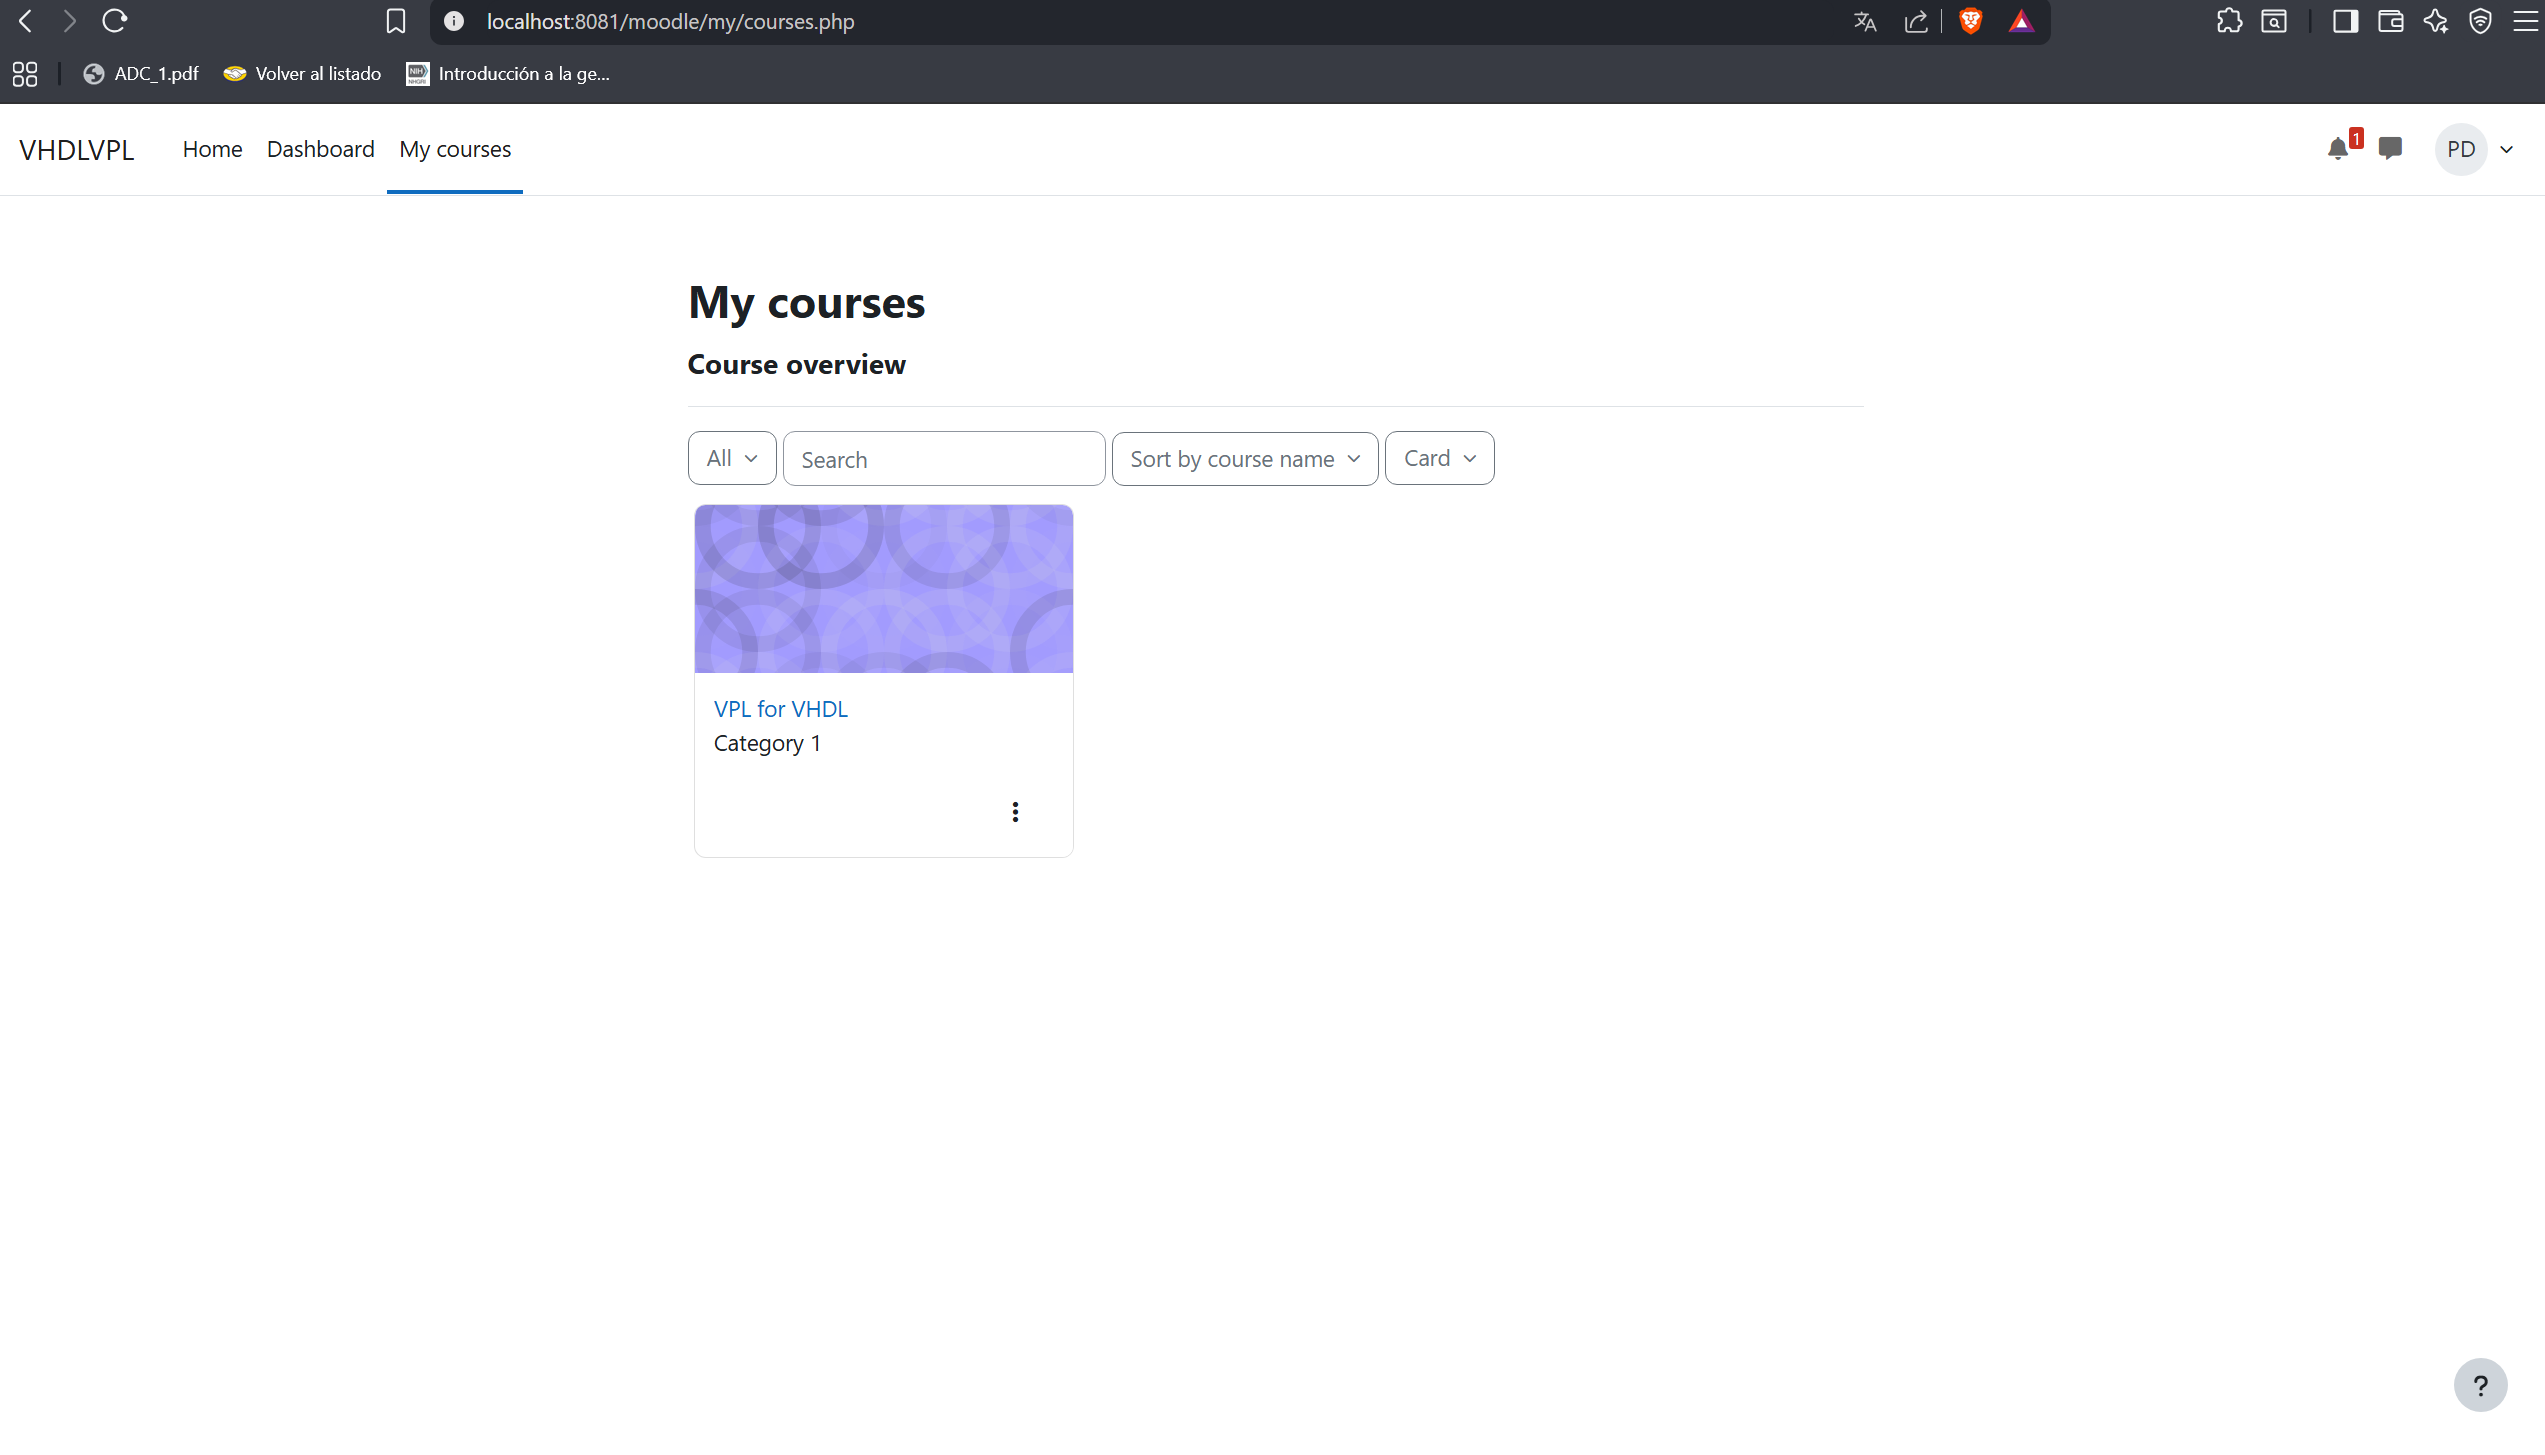
\includegraphics[width=1\textwidth]{moodle/mis_cursos_moodle.png}
\caption{Cursos disponibles en Moodle}
\label{fig:mis-cursos-moodle}
\end{figure}
\begin{stepbox}{2}
  Activar el modo de edición del curso haciendo clic en el botón \menu{Activar edición}.
\end{stepbox}
\begin{figure}[H]
\centering
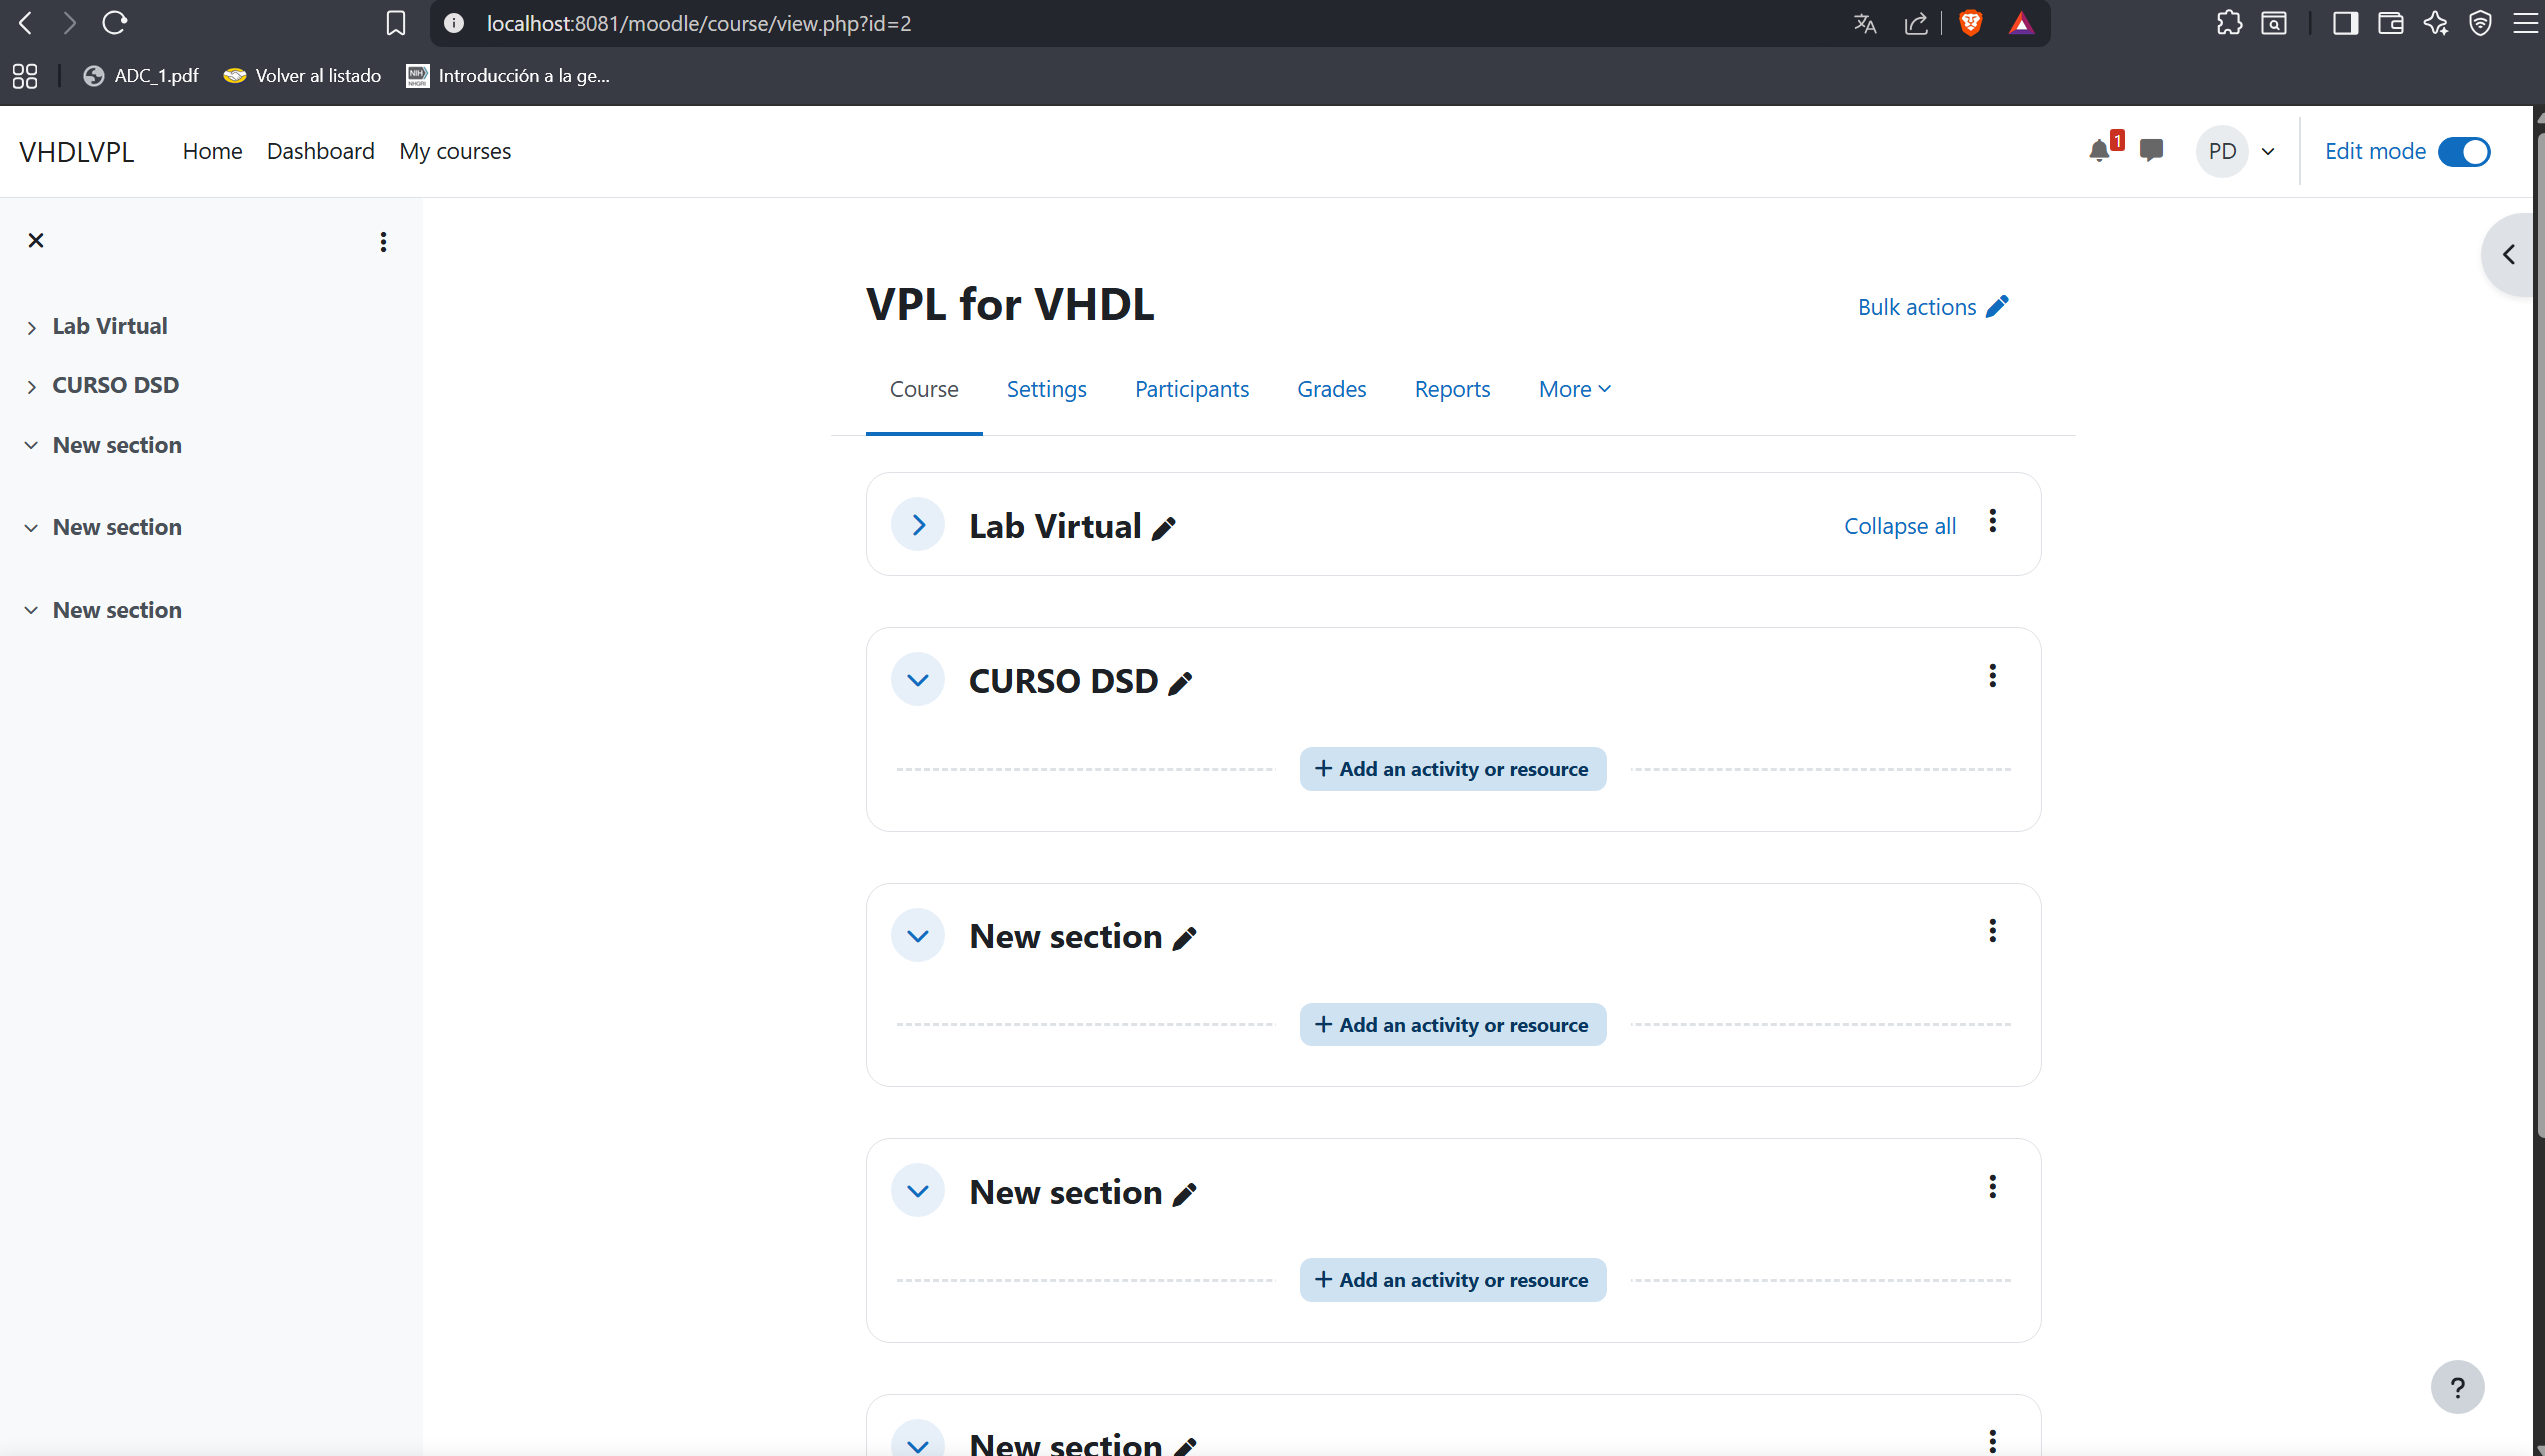
\includegraphics[width=1\textwidth]{moodle/curso_vpl.png}
\caption{Cursos donde se desea agregar la actividad VPL}
\label{fig:curso-vpl}
\end{figure}
\begin{stepbox}{3}
  En la sección del curso donde se desea colocar la actividad, hacer clic en \menu{Añadir una actividad o recurso}.En la ventana emergente, seleccionar \textbf{Virtual Programming Lab (VPL)}.
\end{stepbox}
\begin{figure}[H]
\centering
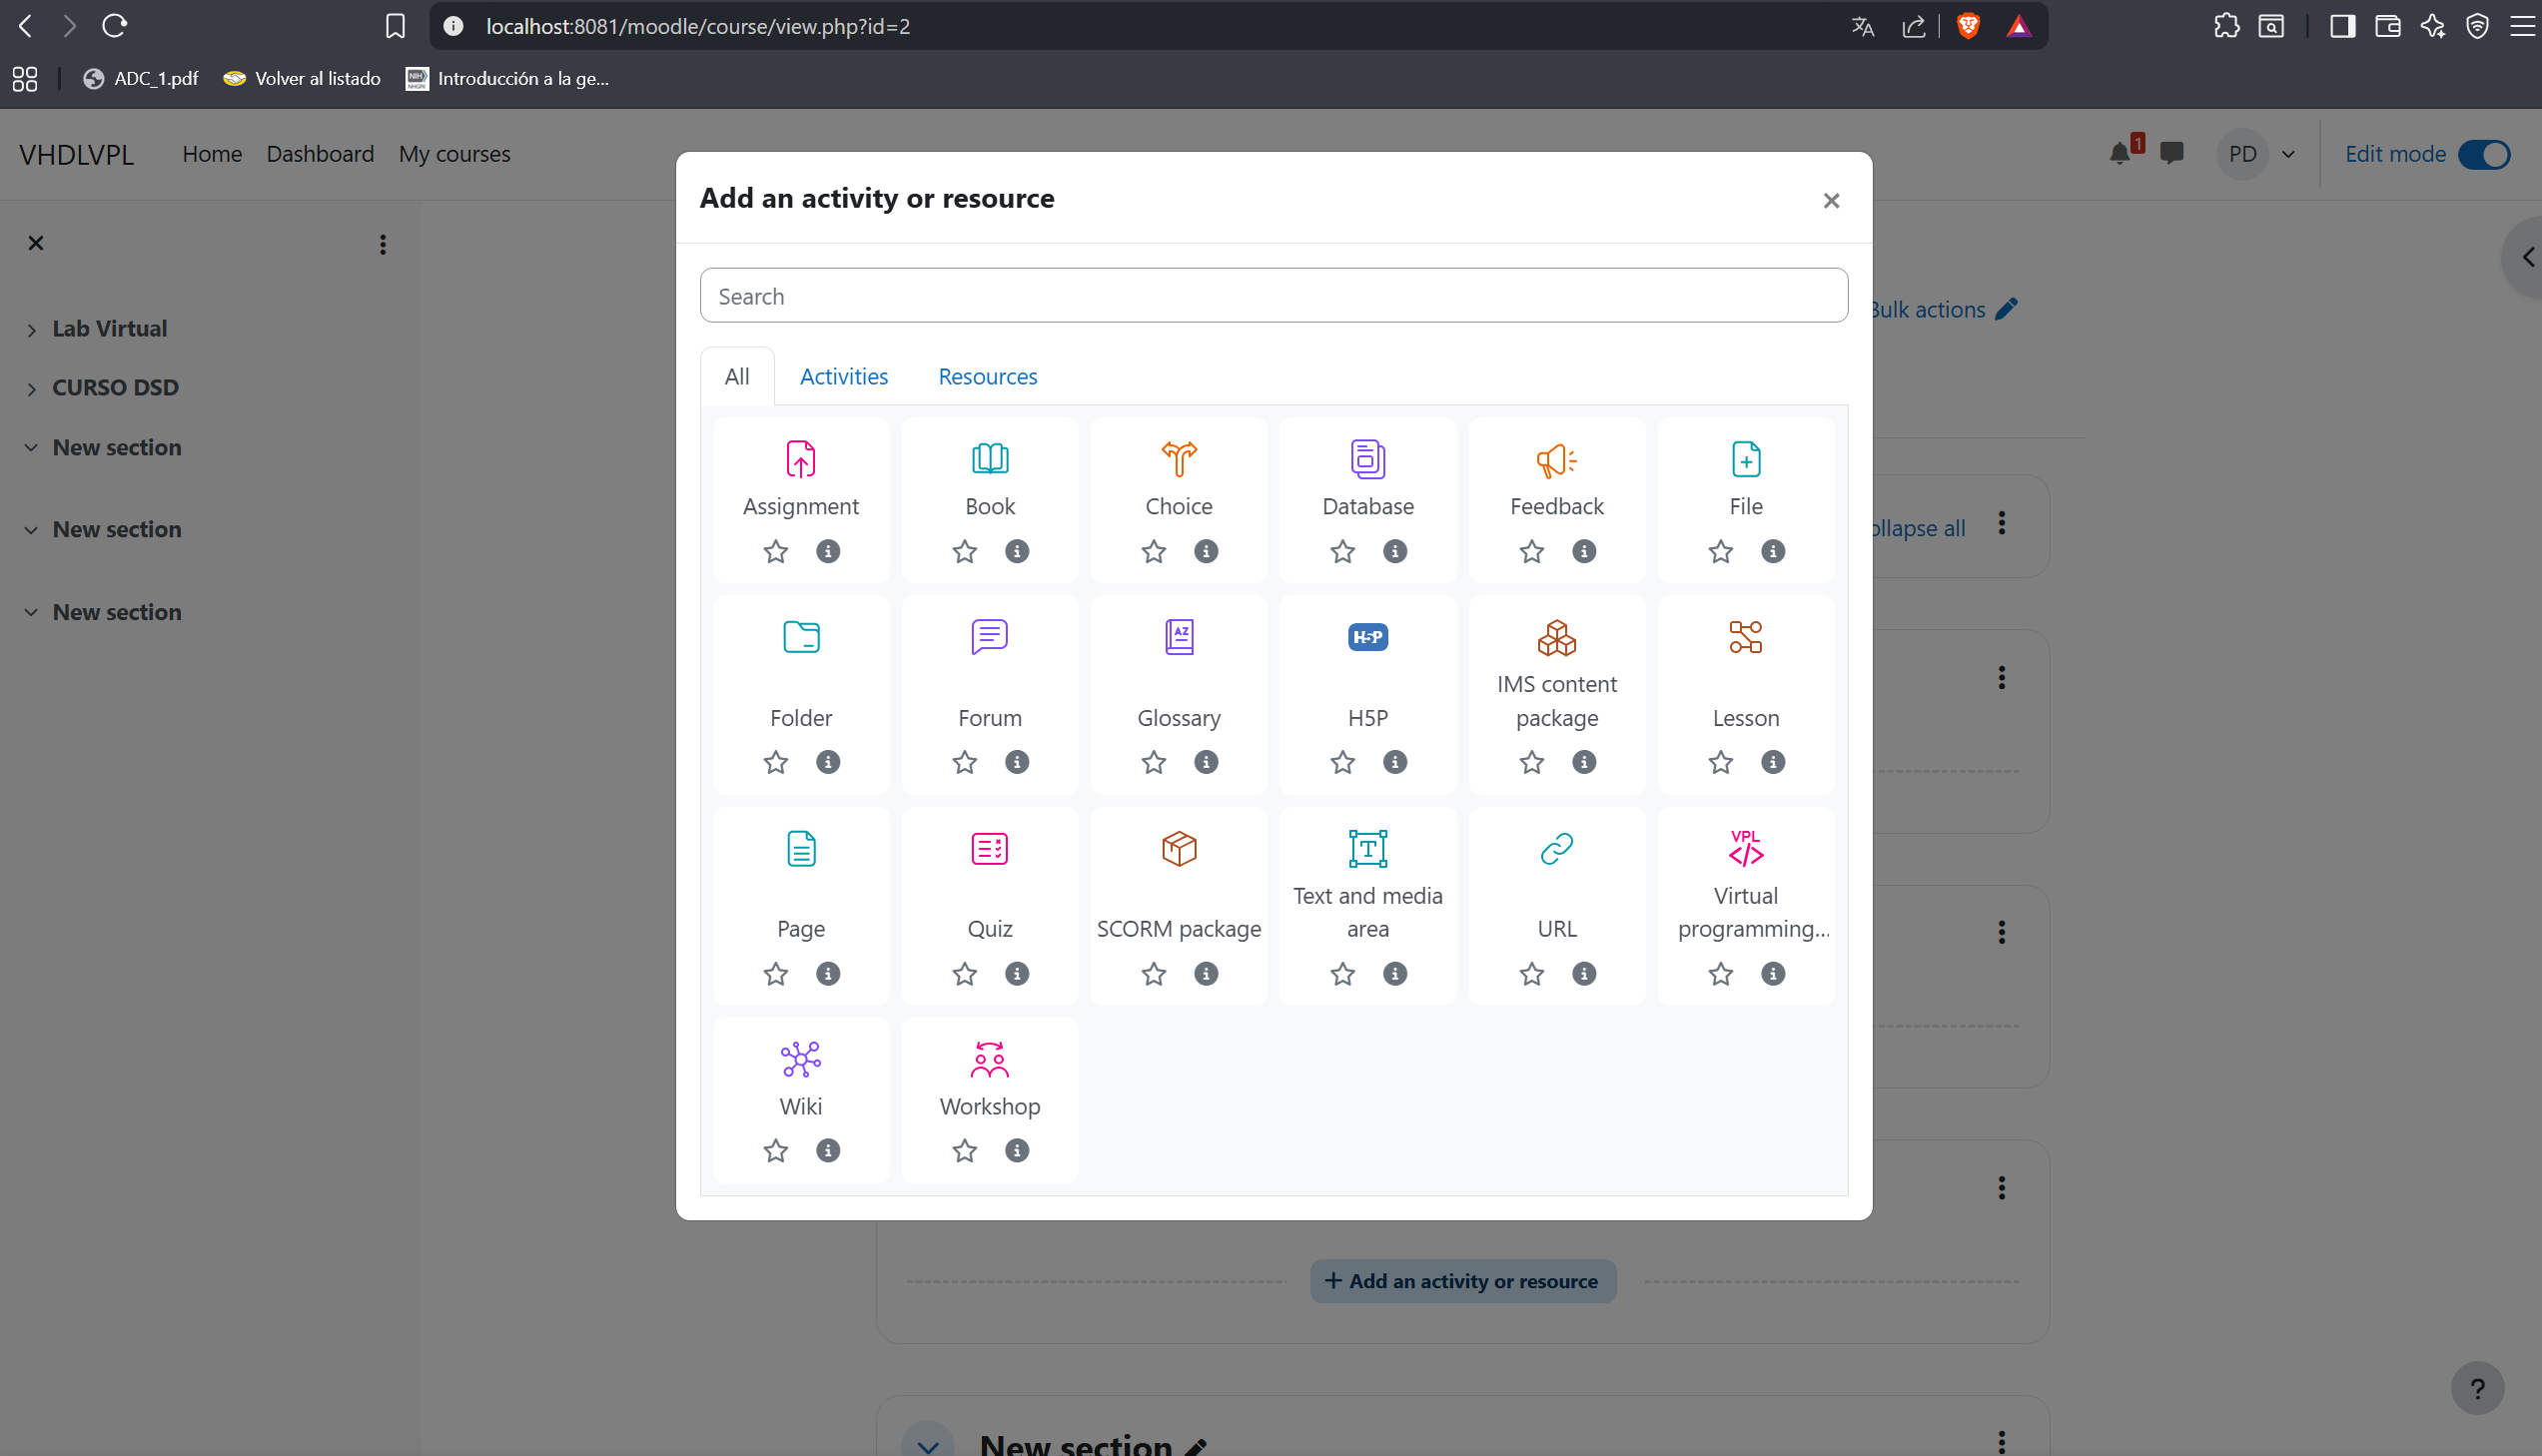
\includegraphics[width=1\textwidth]{vpl/crear_actividad_vpl.png}
\caption{Crear actividad VPL}
\label{fig:crear-actividad-vpl}
\end{figure}

Una vez creada la actividad VPL, se nos muestra una vista para la configuración principal de la actividad, donde se pueden establecer diferentes configuraciones, de las cuales mencionaremos las mas relevantes para el correcto funcionamiento de la actividad, sin embargo, se recomienda revisar cada una de las opciones para personalizar la actividad a las necesidades del curso.

\subsection{Configuraciones generales}
\label{sec:config-generales}
Incluye el nombre de la actividad (obligatorio), una descripción corta y una descripción detallada donde podemos añadir mas recursos (texto, imagenes, videos, etc.).
\begin{figure}[H]
\centering
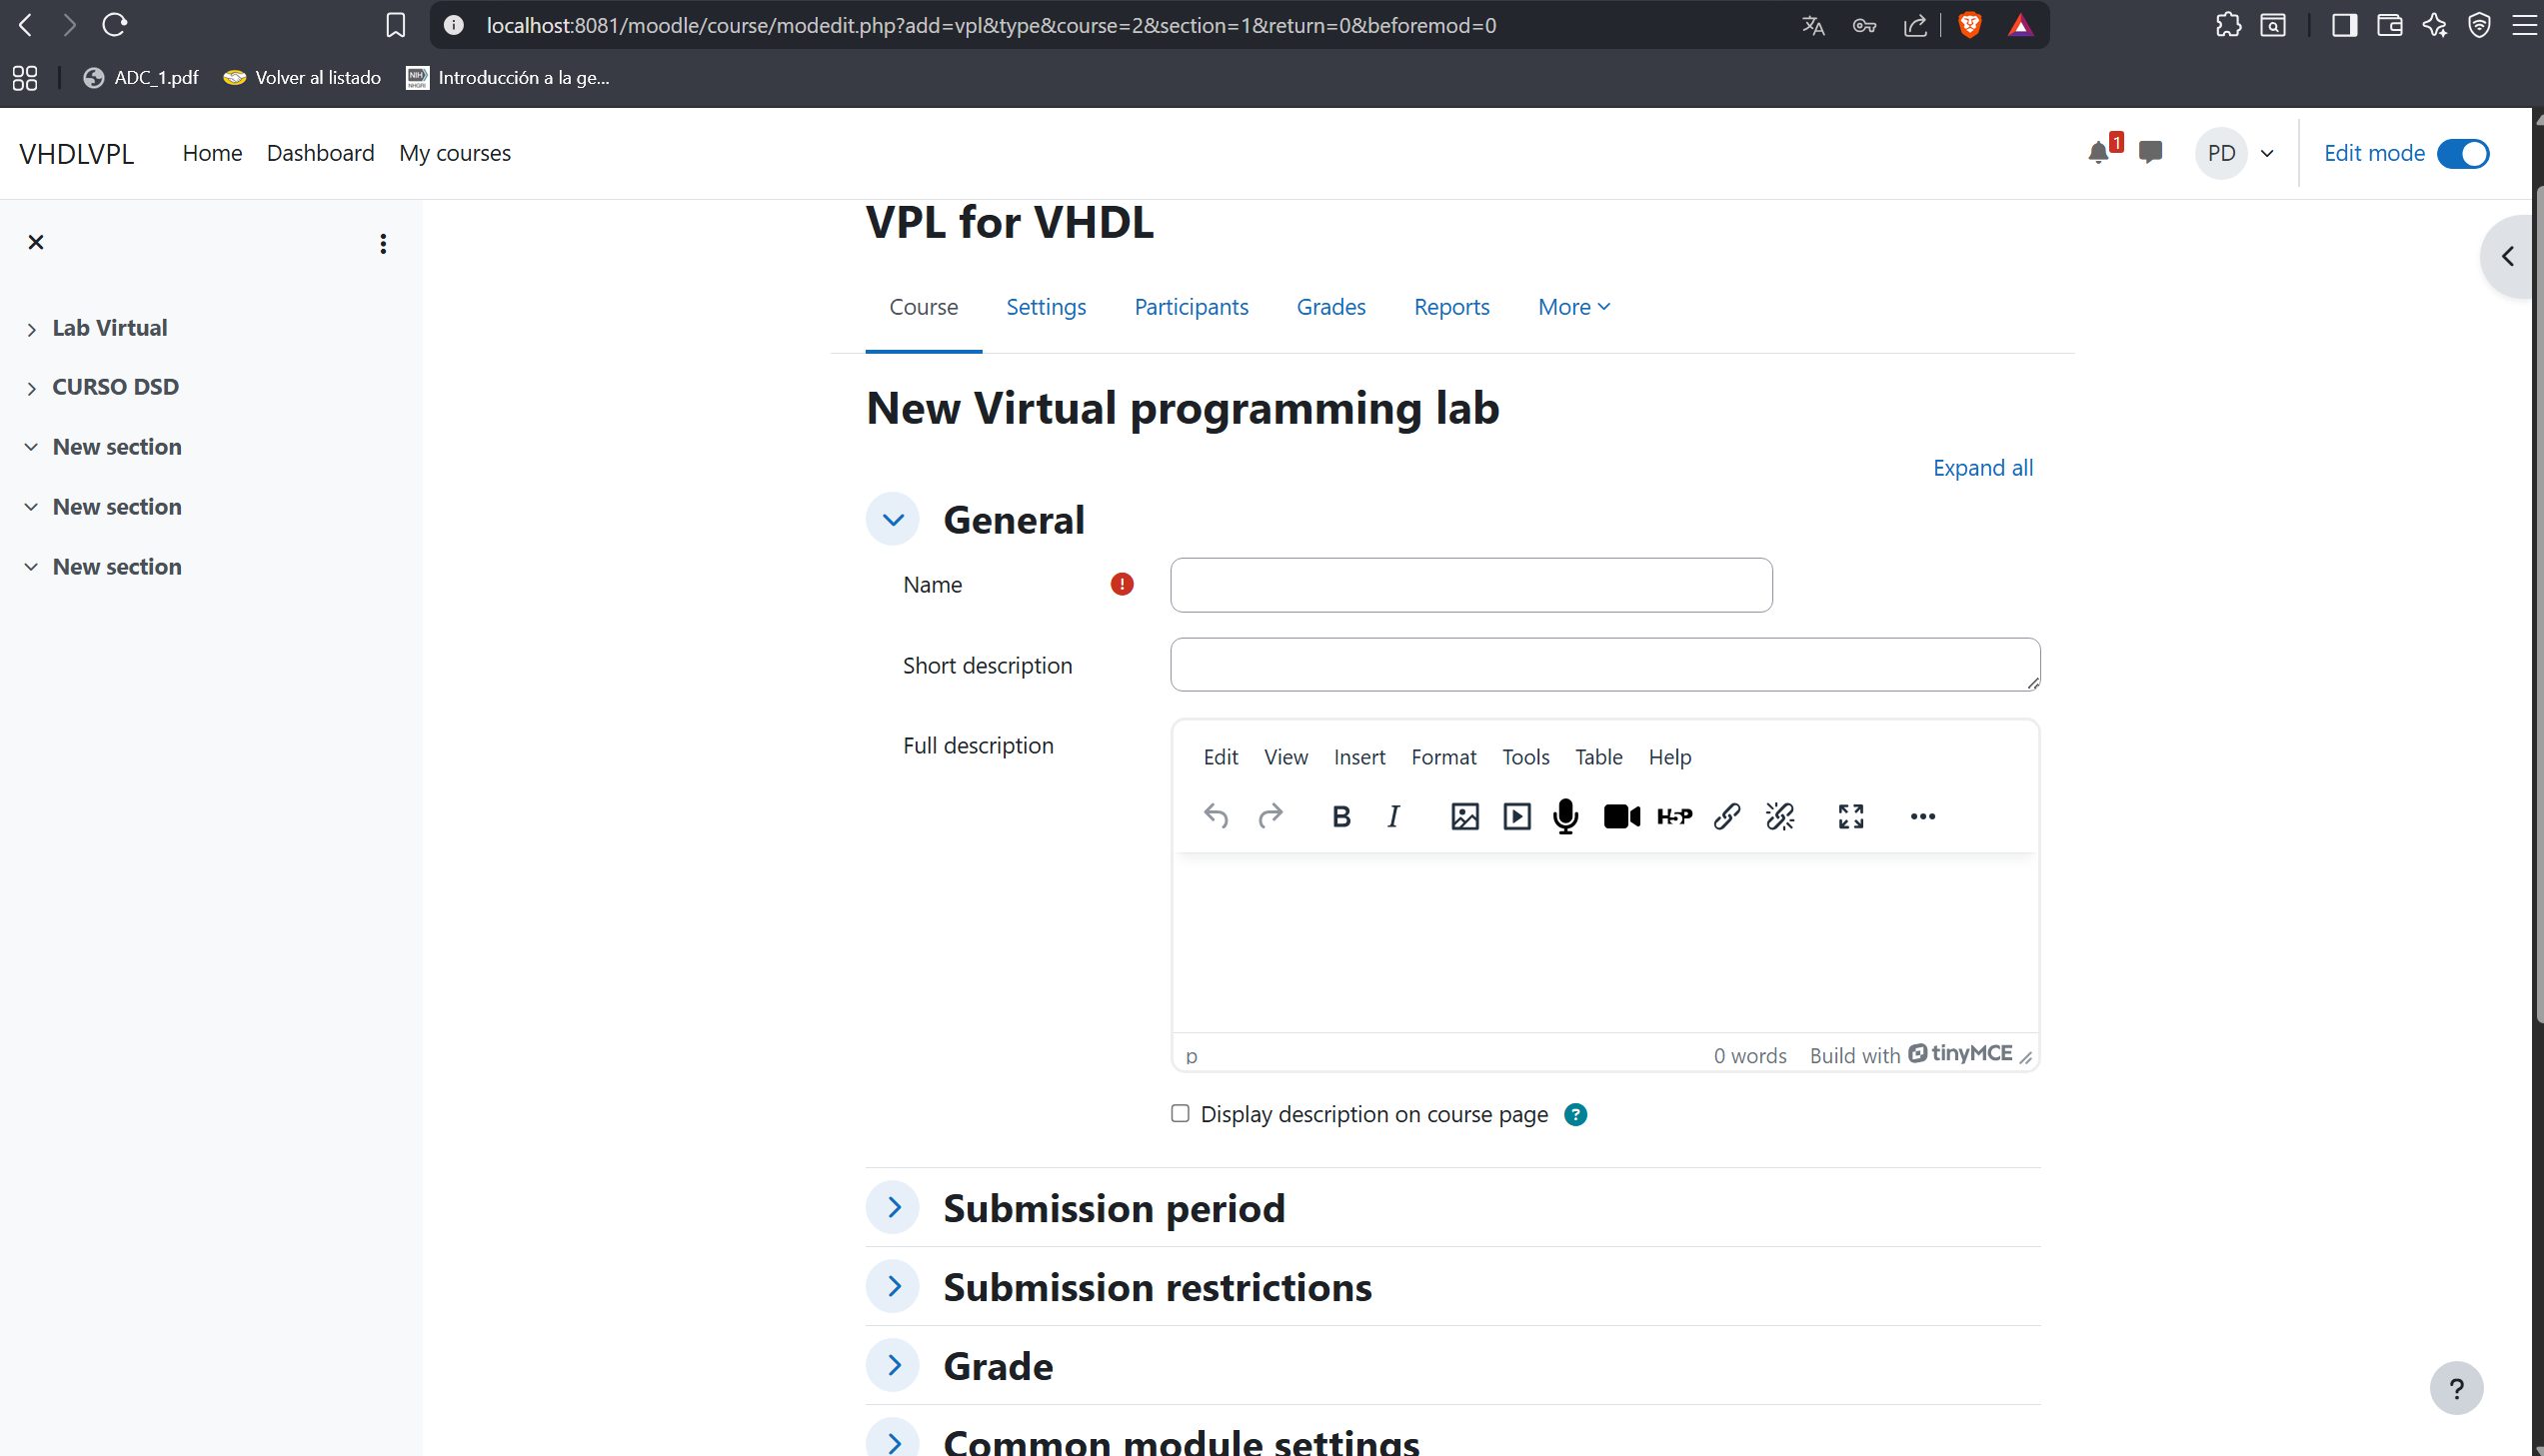
\includegraphics[width=1\textwidth]{vpl/actividad_vpl.png}
\caption{Configuraciones generales de la actividad VPL}
\label{fig:config-generales-vpl}
\end{figure}

\subsection{Restricciones de entrega}
\label{subsec:restricciones}
En esta sección se puedes establecer configuraciones como el numero maximo de archivos que el alumno puede entrgar, el tipo de trabajo (individual o grupal), fecha de entrega, entre otras opciones que pueden ser útiles para controlar la entrega de los trabajos por parte de los alumnos.
Aqui lo mas importante es configurar el numero maximo de archivos que el alumno puede entregar, por default se establecieron 2 archivos maximos, considerando un archivo vhdl fuente y su archivo testbench generado, sin embargo, dependiendo de la actividad se pueden establecer mas archivos maximos para que el alumno pueda entregar archivos adicionales (por ejemplo, un archivo de texto con una explicación del diseño o un diagrama del circuito).
\begin{figure}[H]
\centering
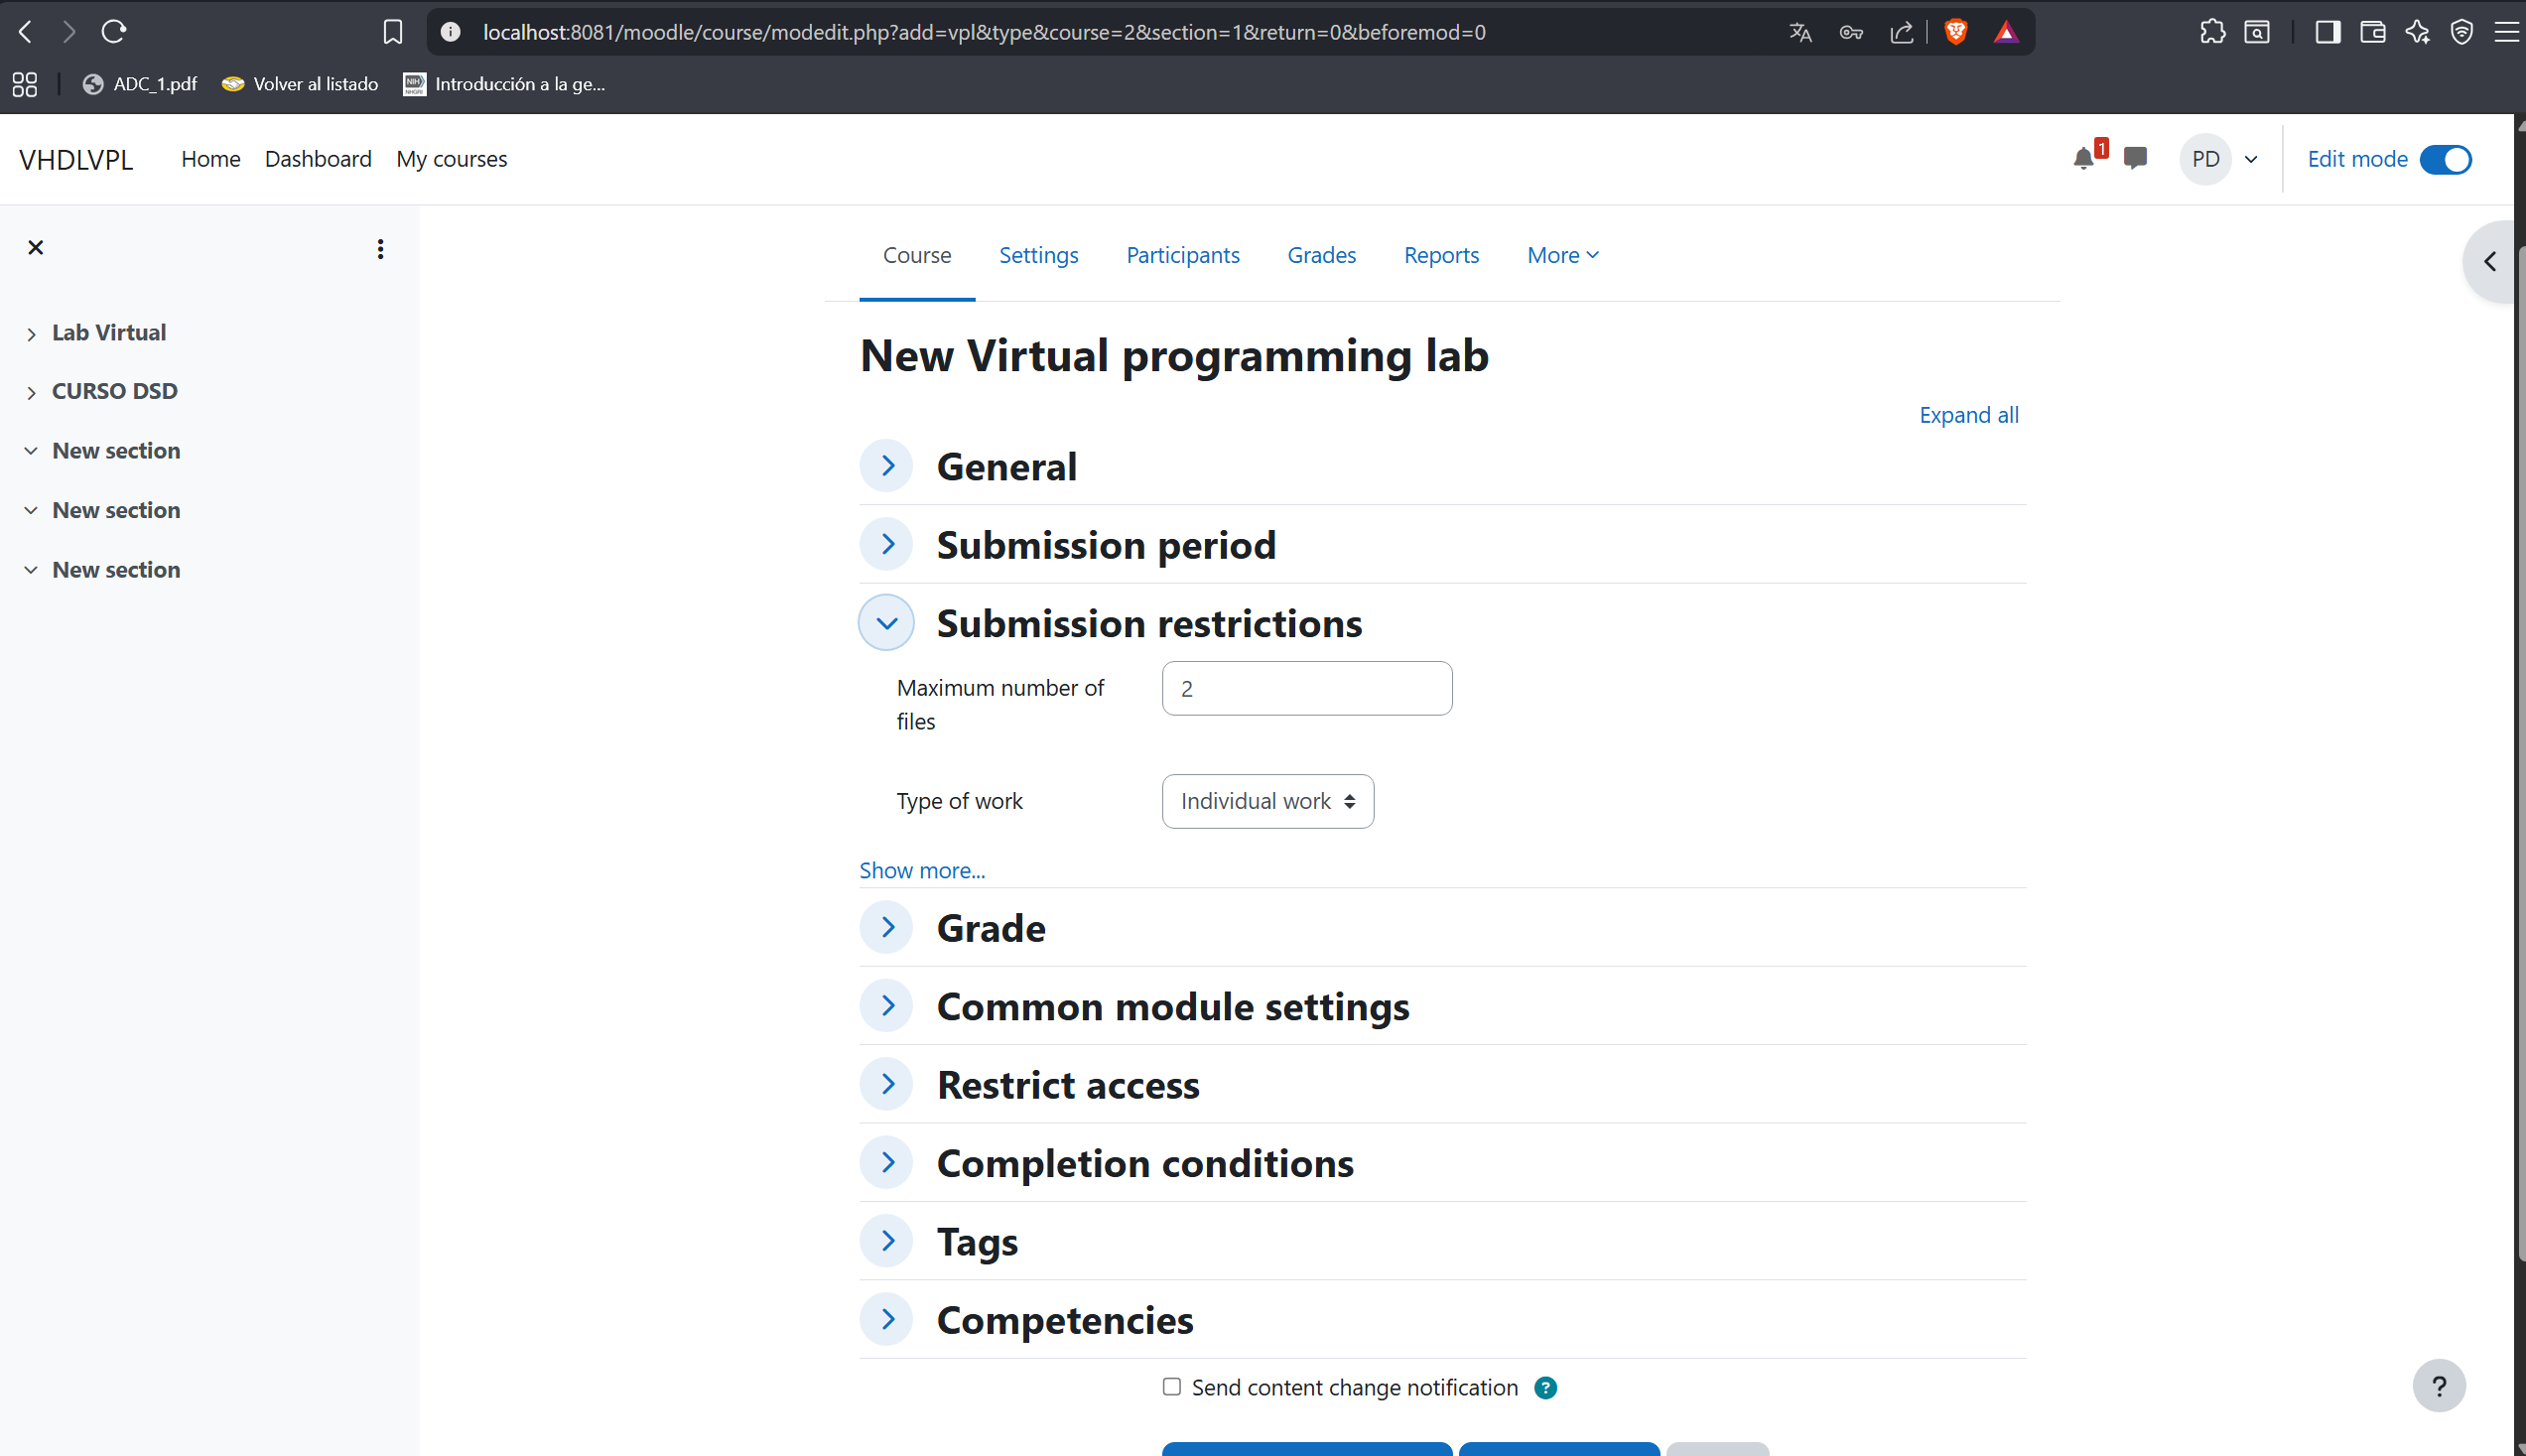
\includegraphics[width=1\textwidth]{vpl/restricciones_actividad_vpl.png}
\caption{Restricciones de entrega en la actividad VPL}
\label{fig:restricciones-vpl}
\end{figure}

\subsection{Otras configuraciones}
\label{subsec:config-otras}
EL VPL es un plugin muy completo que ofrece muchas opciones de configuración, por lo que se recomienda revisar cada una de las secciones para personalizar la actividad a las necesidades del curso, sin embargo, se recomienda revisar la  documentacion propia de VPL for Moodle para  saber mas acerca de las otras configuraciones.


Una vez configurada la activisdad, se debe guardar los cambios para que la actividad quede disponible para los alumnos.
\begin{figure}[H]
\centering
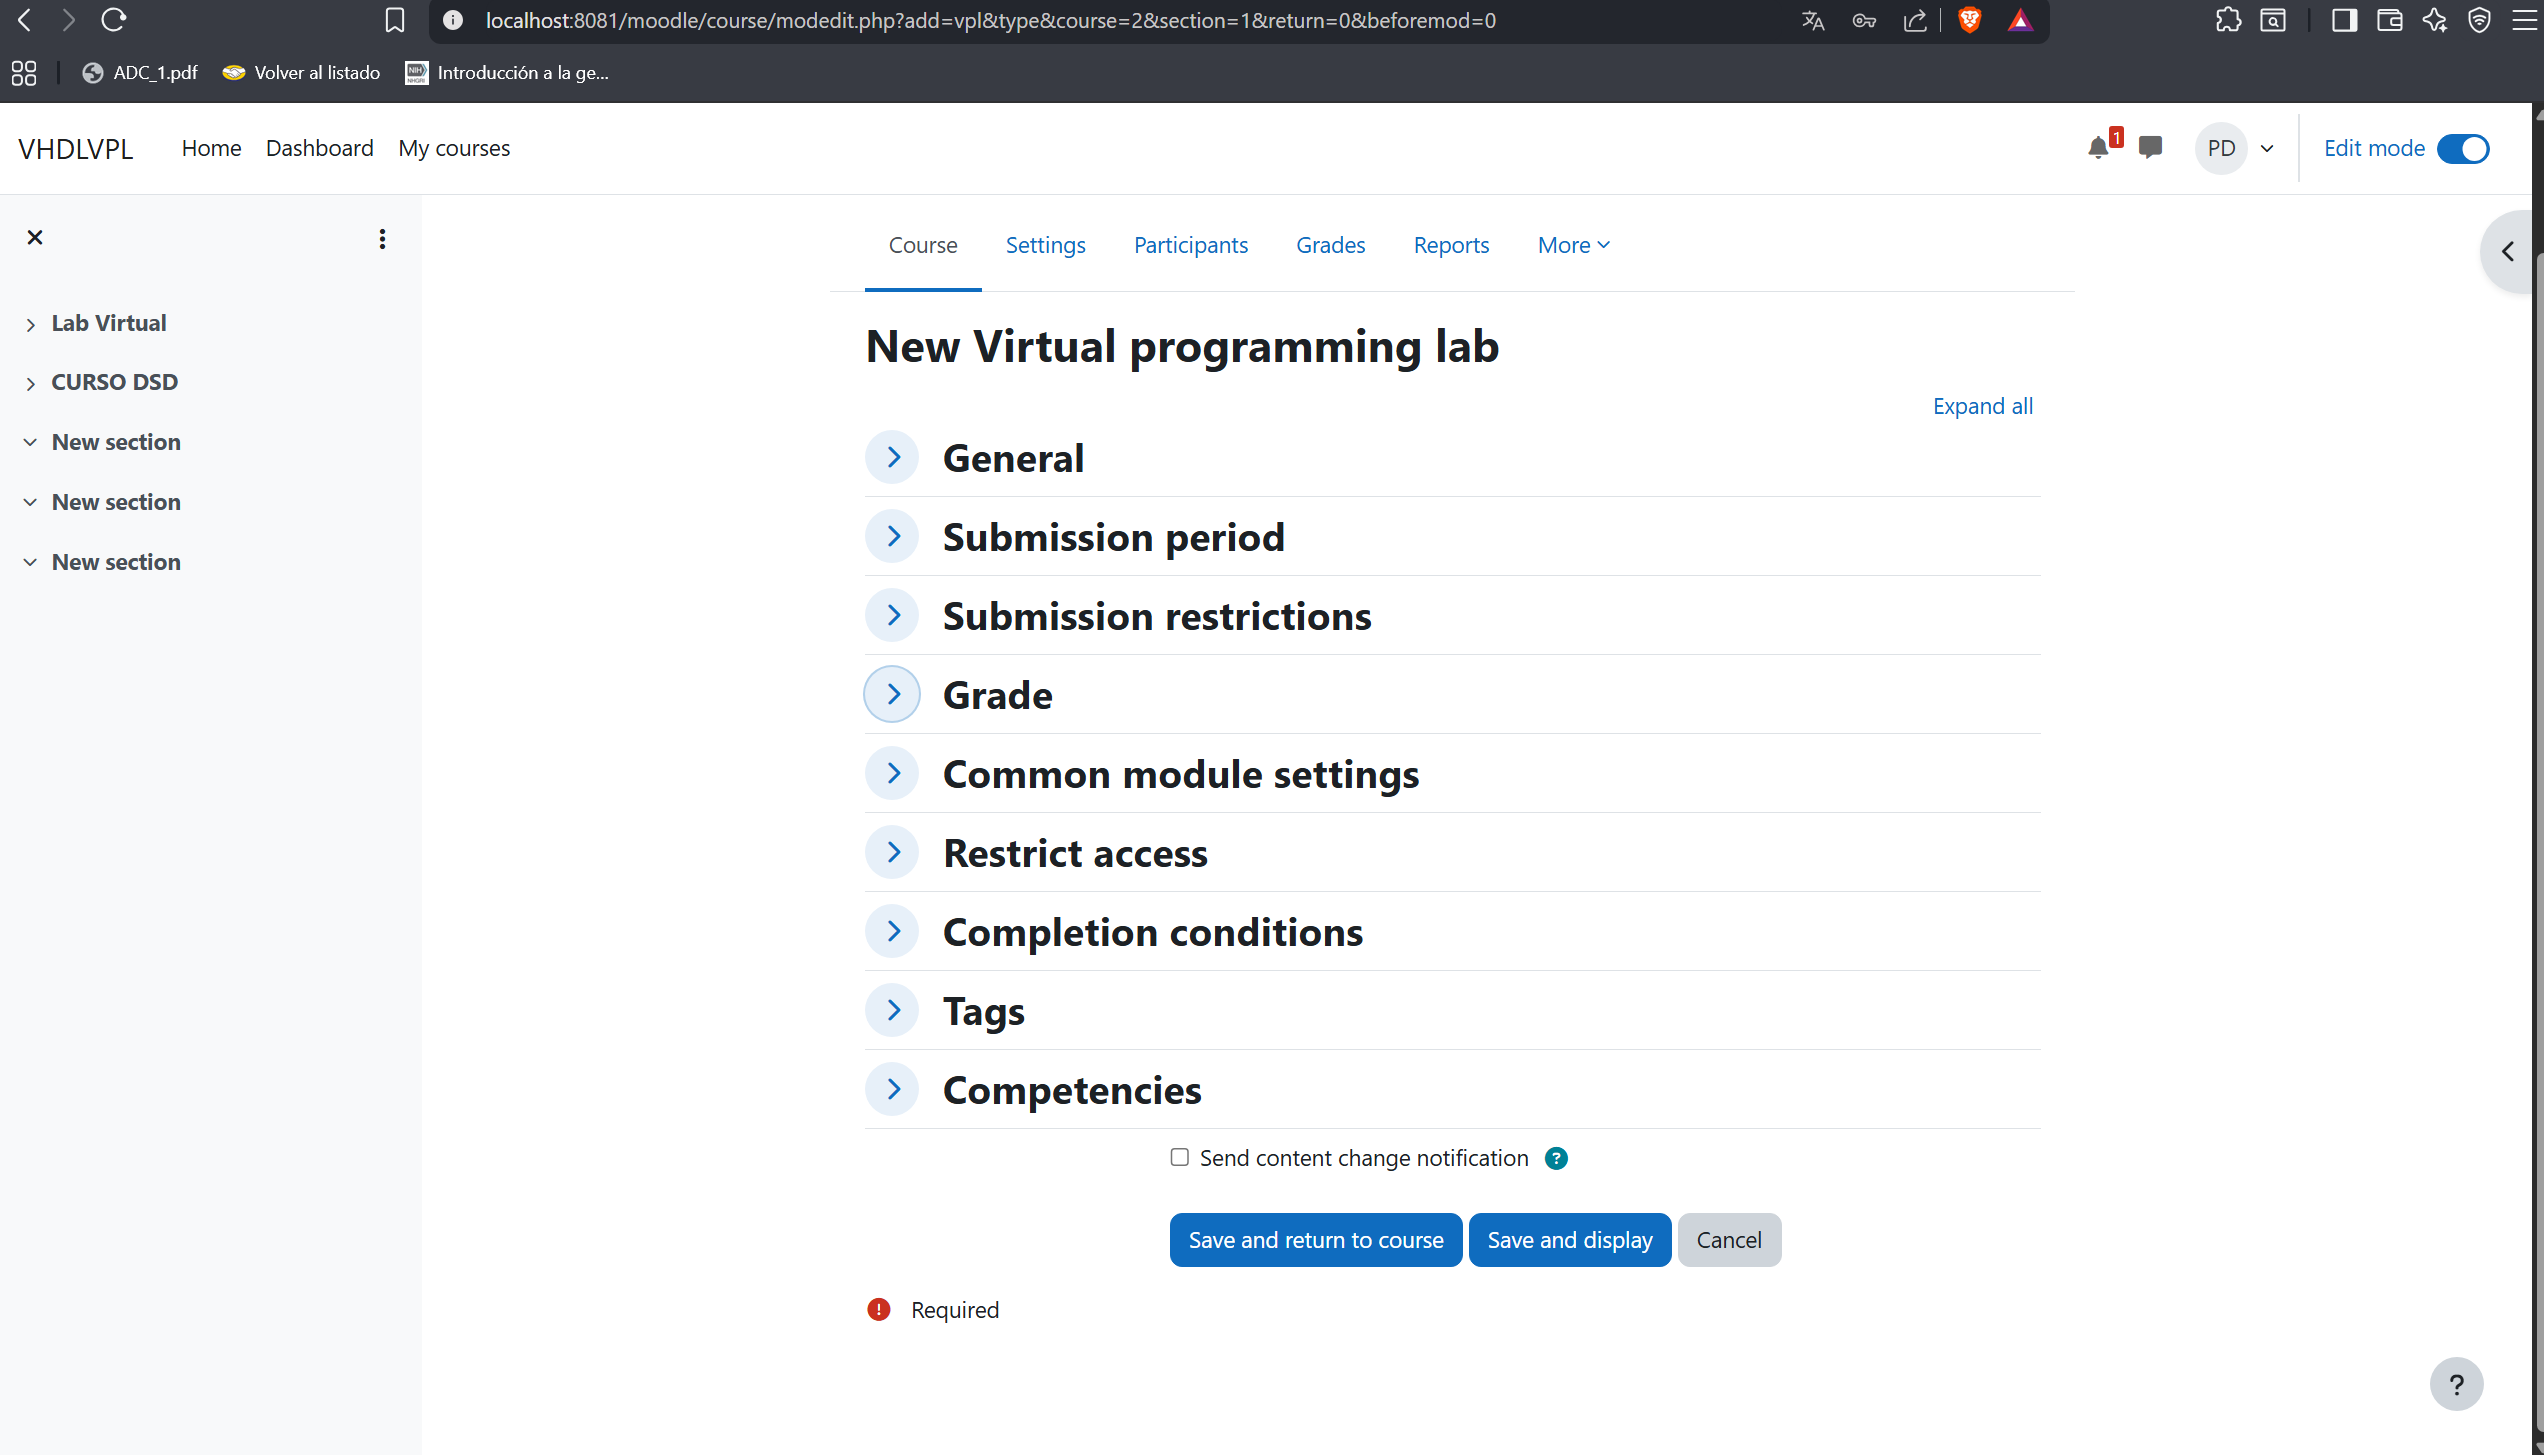
\includegraphics[width=1\textwidth]{vpl/guardar_actividad_vpl.png}
\caption{Guardar cambios en la actividad VPL}
\label{fig:guardar-actividad-vpl}
\end{figure}

Una vez guardadas las configuraciones establecidas, la actividad deberia verse como en la siguiente imagen:
\begin{figure}[H]
\centering
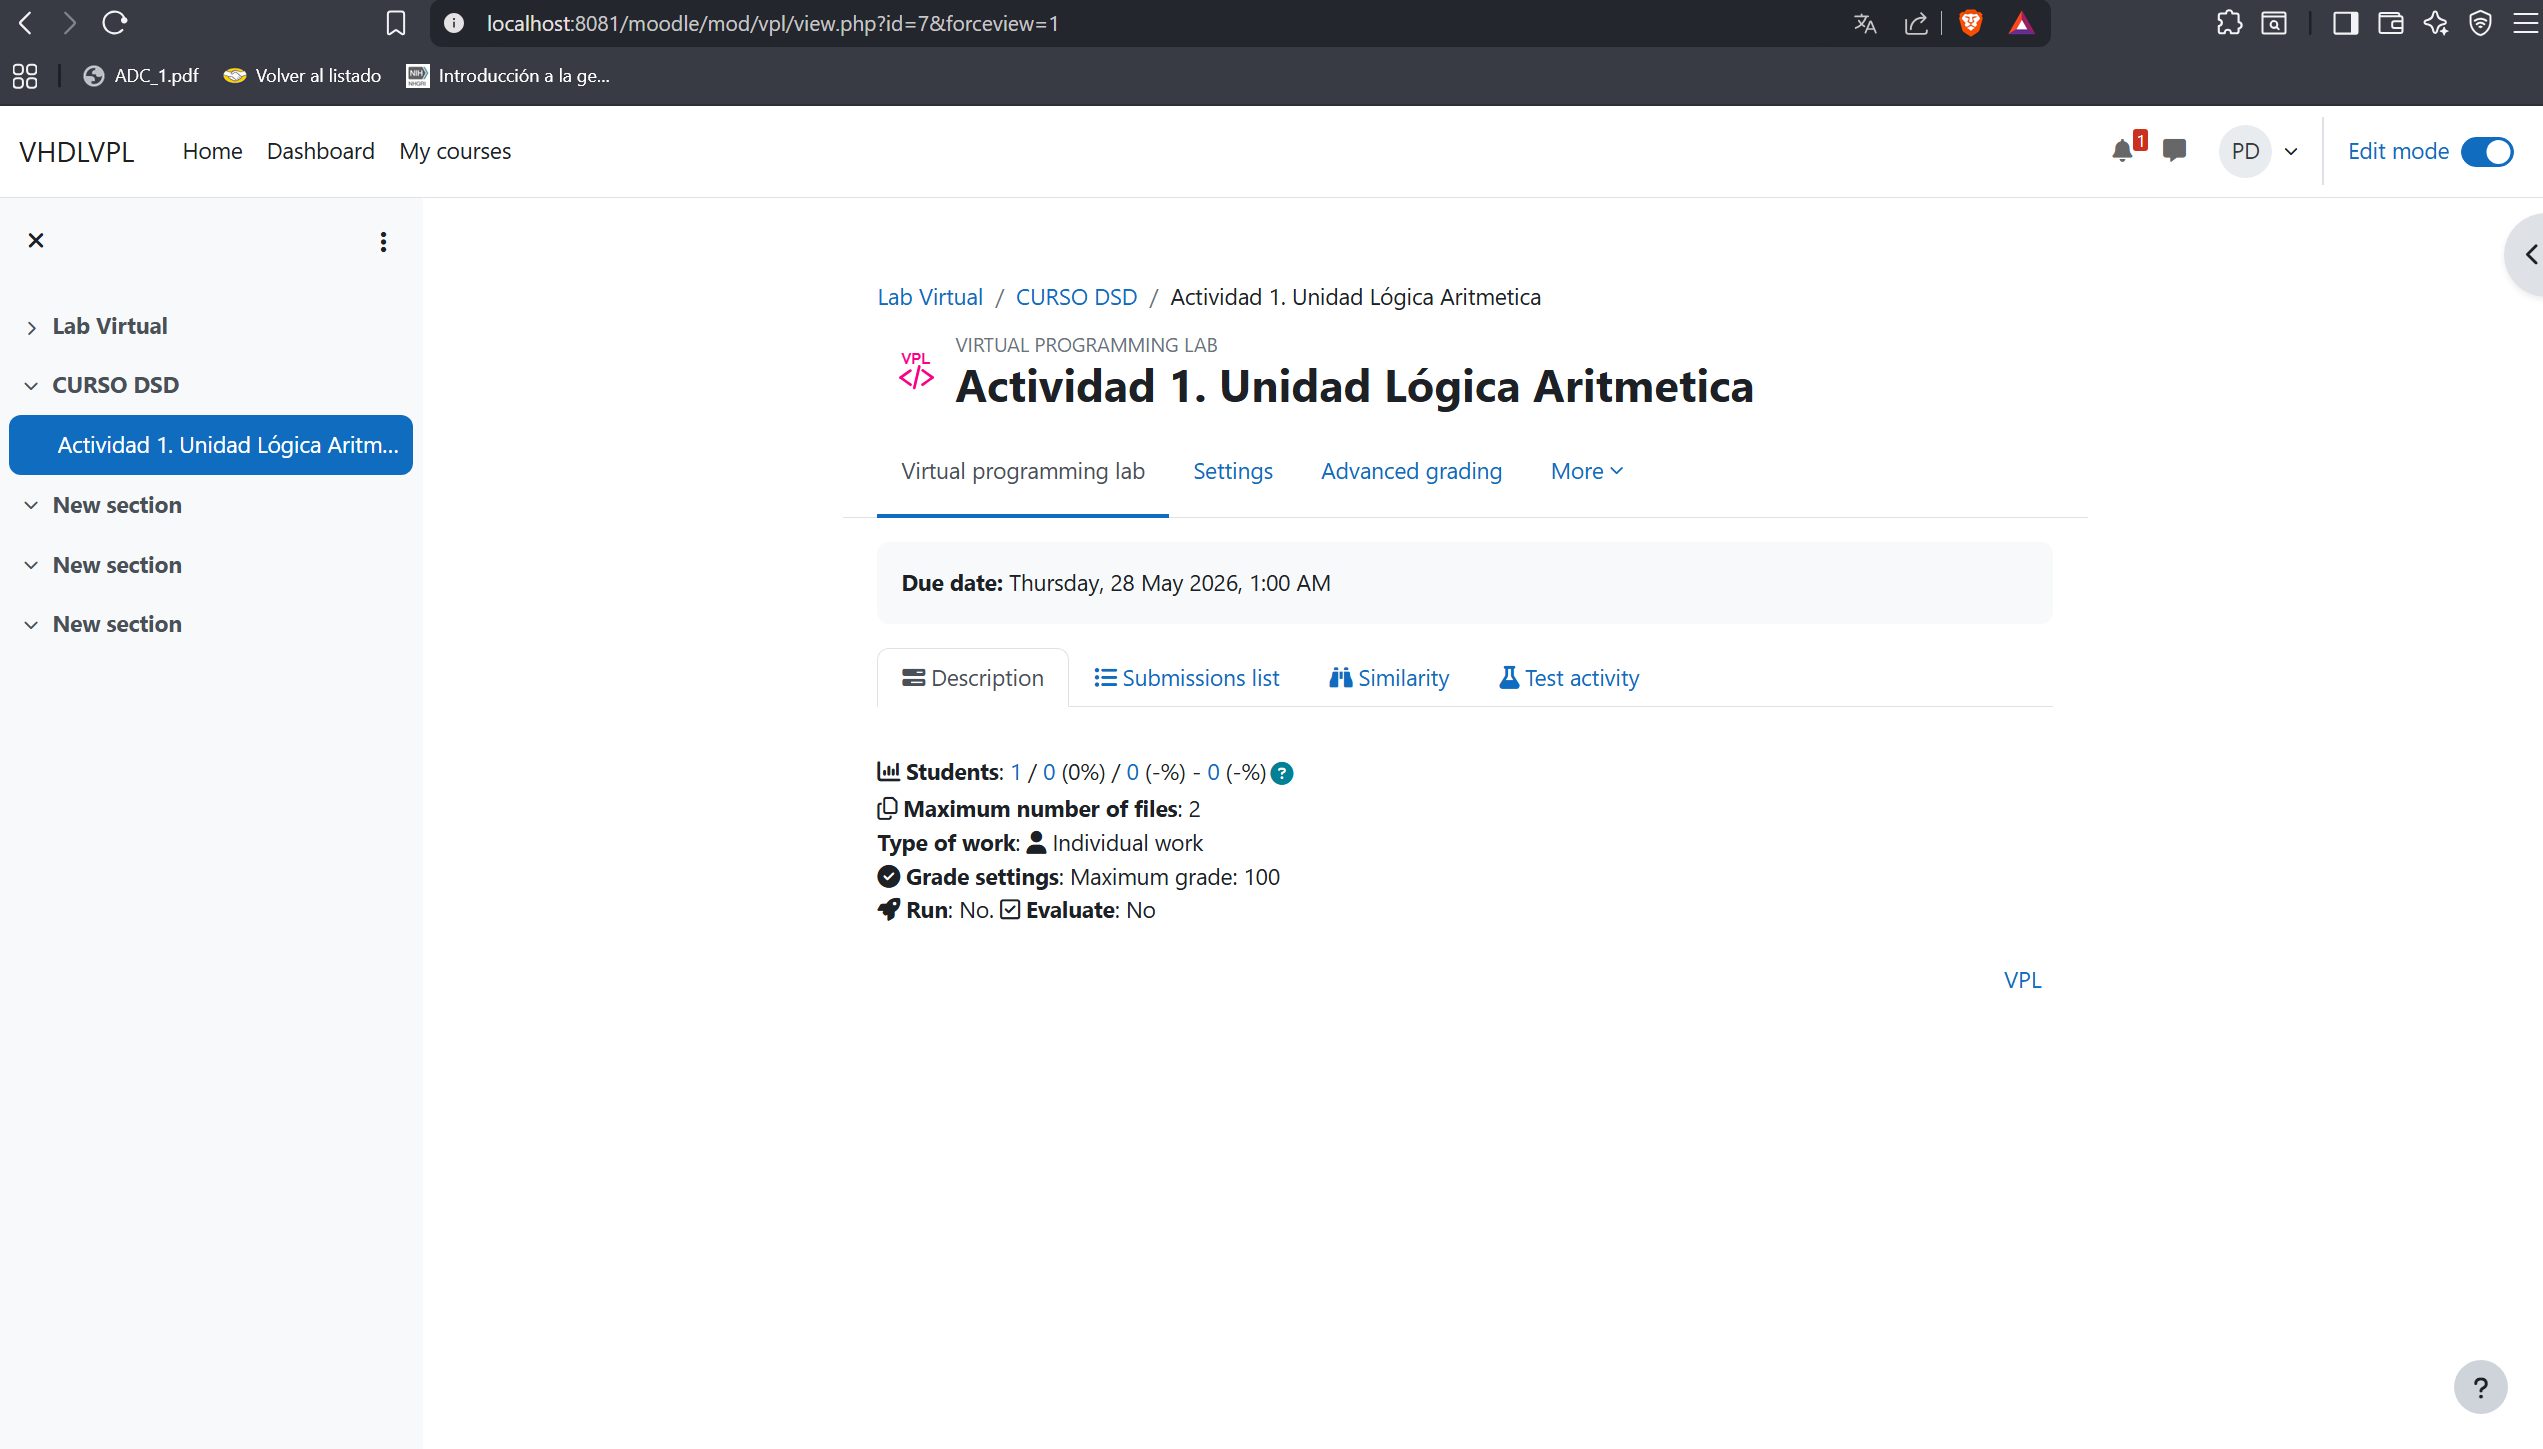
\includegraphics[width=1\textwidth]{vpl/overview_actividad_vpl.png}
\caption{Visión general de la actividad VPL}
\label{fig:vista_general}
\end{figure}

% ── Capítulo 9 ──────────────────────────────────────────────
\chapter{Acciones Permitidas}
\label{ch:acciones}
En esta sección se describen como configurar las acciones que ofrece el entorno de VPL, esto respecto a la ejecución, depuración y evaluación de los diseños VHDL entregados por los alumnos.
Es importante configurar esta sección una vez creada la actividad, ya que si visualizamos la imagen \ref{fig:vista_general}, observamos que por se visualiza la acción  RUN habilitada y Evaluate deshabilitada, 
por lo que hay que configurar las  acciones para permitir o no al alumno usarlas.

\section{Tipos de acciones en VPL}
\label{sec:tipos-acciones}
En el laboratorio virtual de VPL, existen 5 tipos principales de acciones  que se pueden configurar para los alumnos:
\begin{itemize}
  \item \textbf{Run (Ejecutar):} Permite a los alumnos ejecutar su código VHDL para verificar su funcionamiento básico. Esta acción generalmente compila y simula el diseño, mostrando los resultados de la simulación.
  \item \textbf{Debug (Depurar):} Permite a los alumnos depurar su código VHDL, lo que puede incluir la visualización de formas de onda, inspección de señales y análisis detallado del comportamiento del diseño durante la simulación.
  \item \textbf{Evaluate (Evaluar):} Permite a los alumnos enviar su diseño para evaluación automática, donde se ejecutan casos de prueba predefinidos para verificar la corrección del diseño y asignar una calificación basada en los resultados. 
  \item \textbf{Remote Lab (Laboratorio Remoto):} Permite conectarse al laboratorio remoto de FPGA'S.
  \item \textbf{Testbench (Generar Testbench):} Permite a los alumnos generar automáticamente un testbench básico para su diseño VHDL, lo que facilita la simulación y verificación de su código.
\end{itemize}

\section{Configurar acciones disponibles para el alumno}
\label{sec:config-acciones}
Para habilitar o deshabilitar estas acciones para los alumnos, se deben seguir los siguientes pasos:
\begin{stepbox}{1}
  Ingresar a la actividad VPL creada y hacer clic en el botón \menu{MAS / More} para que se desplieguen mas opciones del VPL.
\end{stepbox}
\begin{figure}[H]
\centering
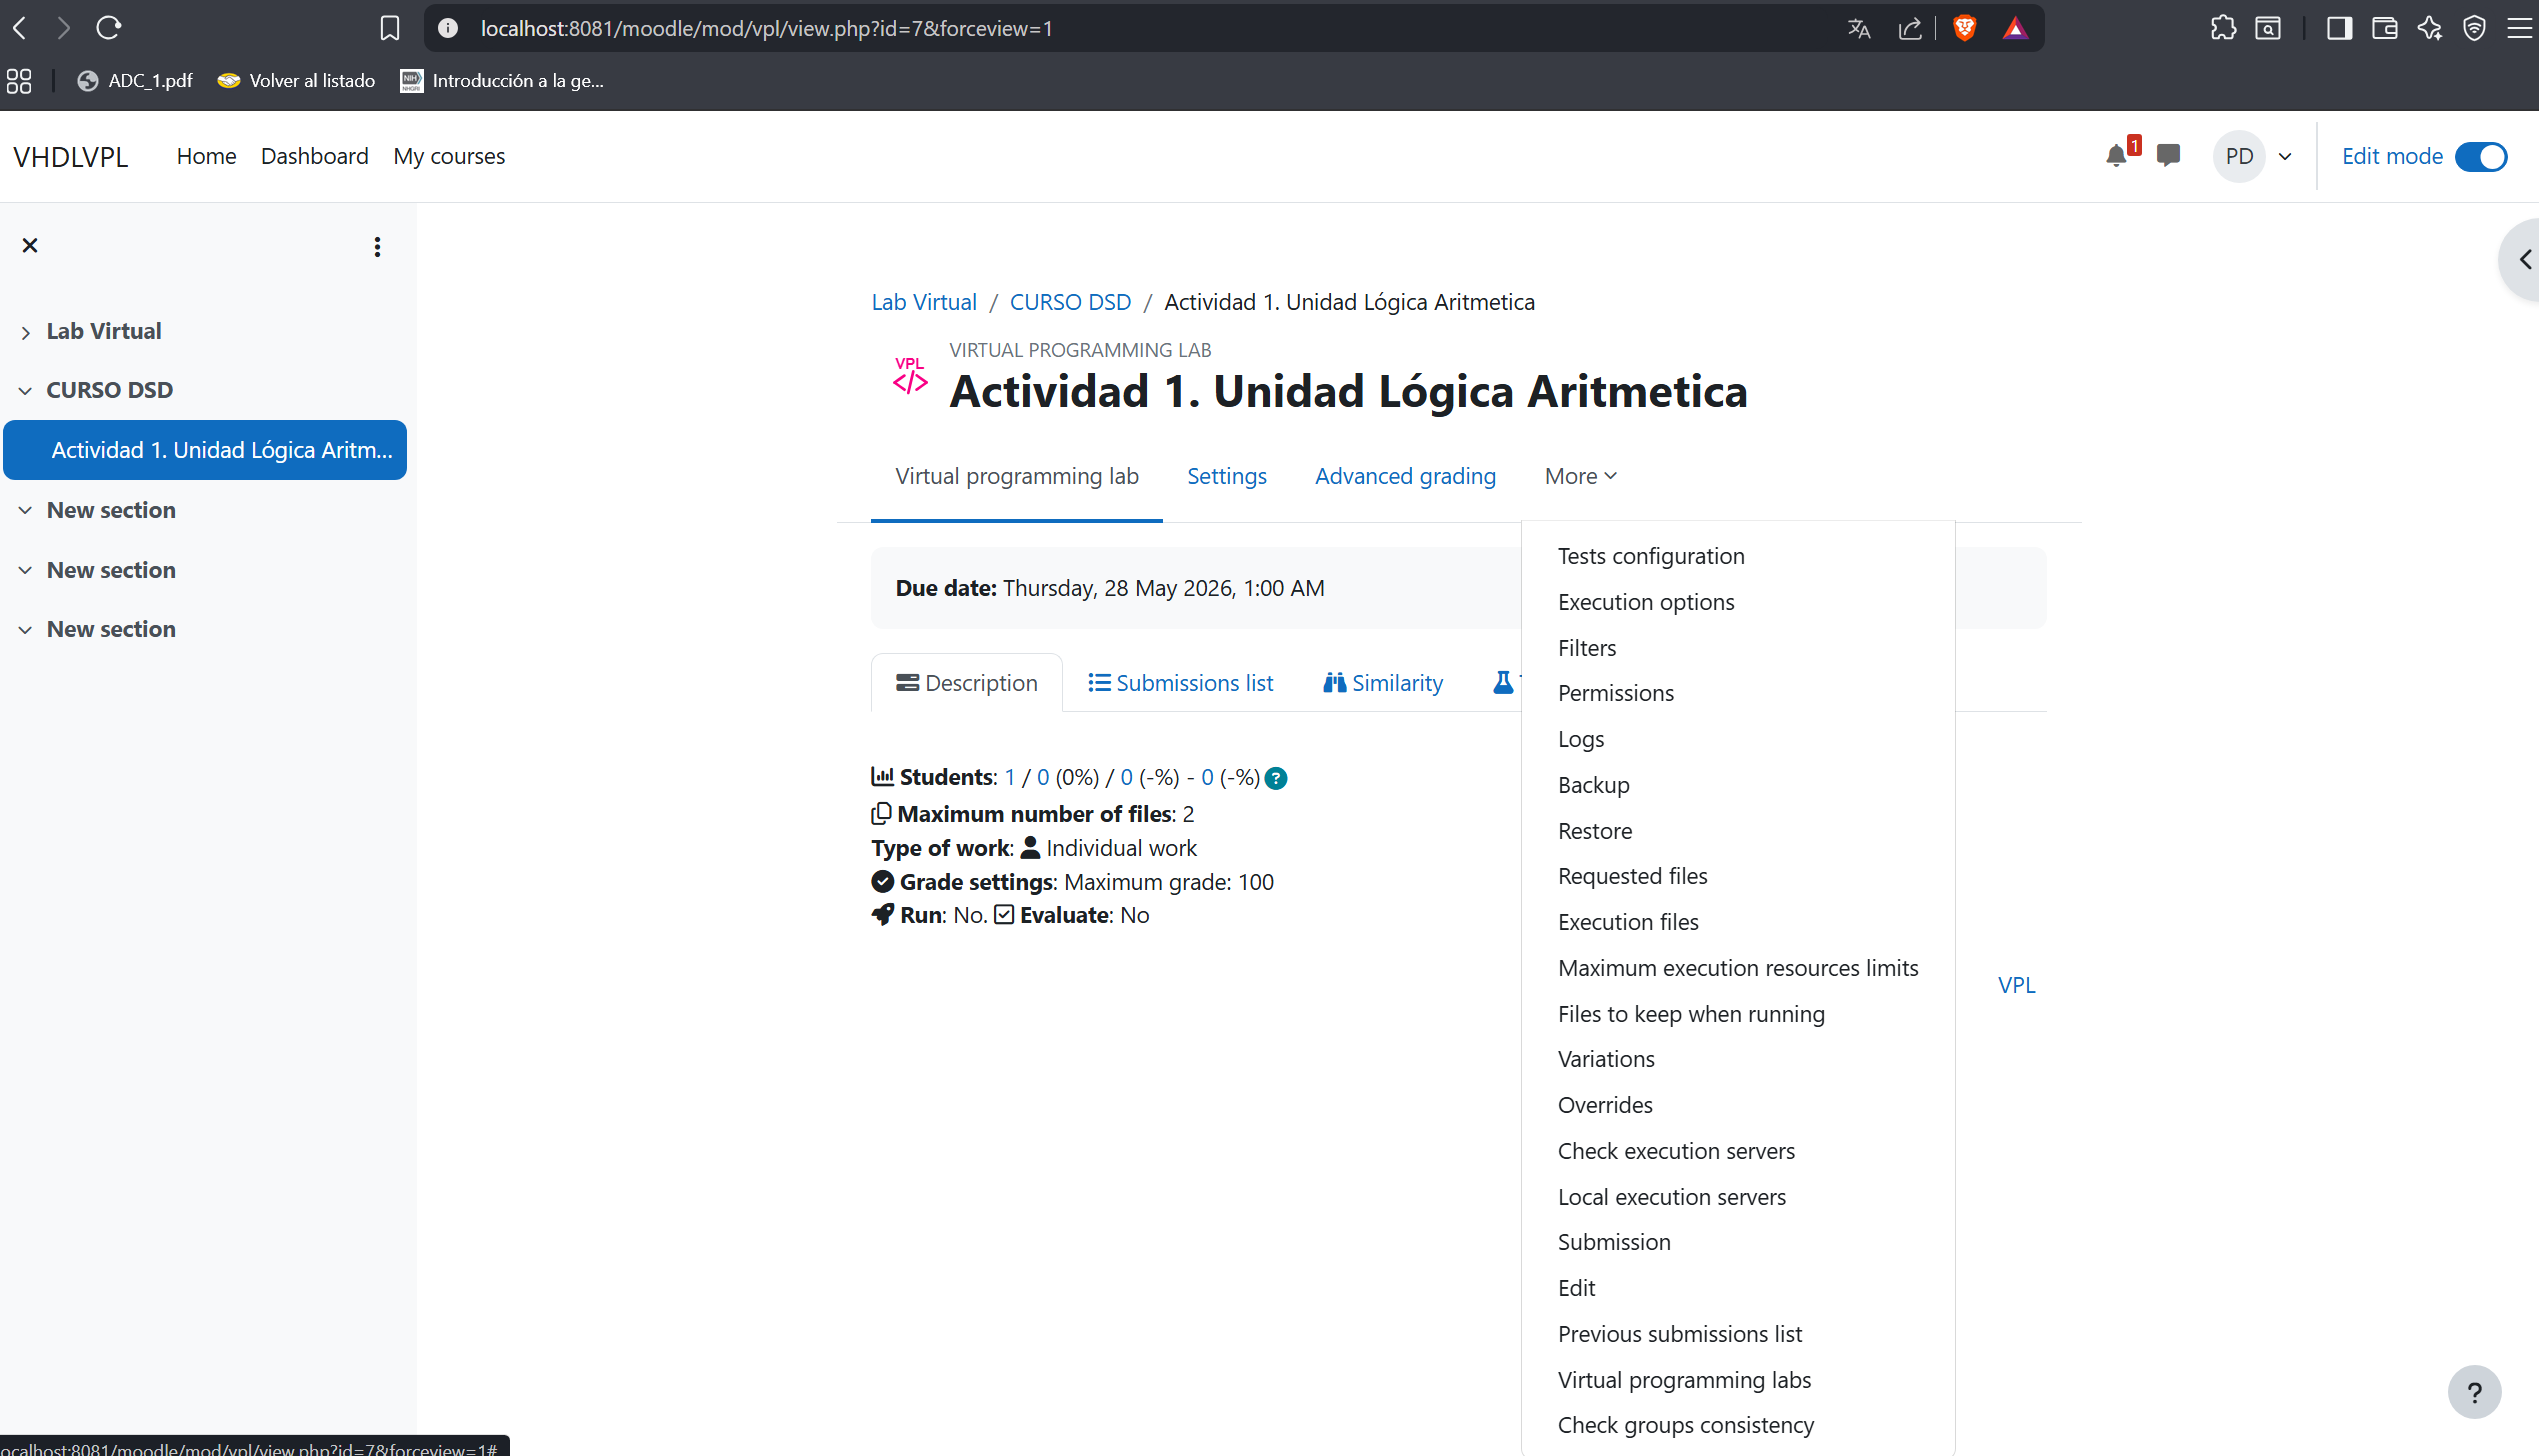
\includegraphics[width=1\textwidth]{profesor/mas_actividad_vpl.png}
\caption{Mas configuraciones de la actividad VPL}
\label{fig:mas-actividad-vpl}
\end{figure}
\begin{stepbox}{2}
  En la sección de \textbf{Acciones de ejecución}, seleccionar las acciones que se desean habilitar para los alumnos.
\end{stepbox}
\begin{figure}[H]
\centering
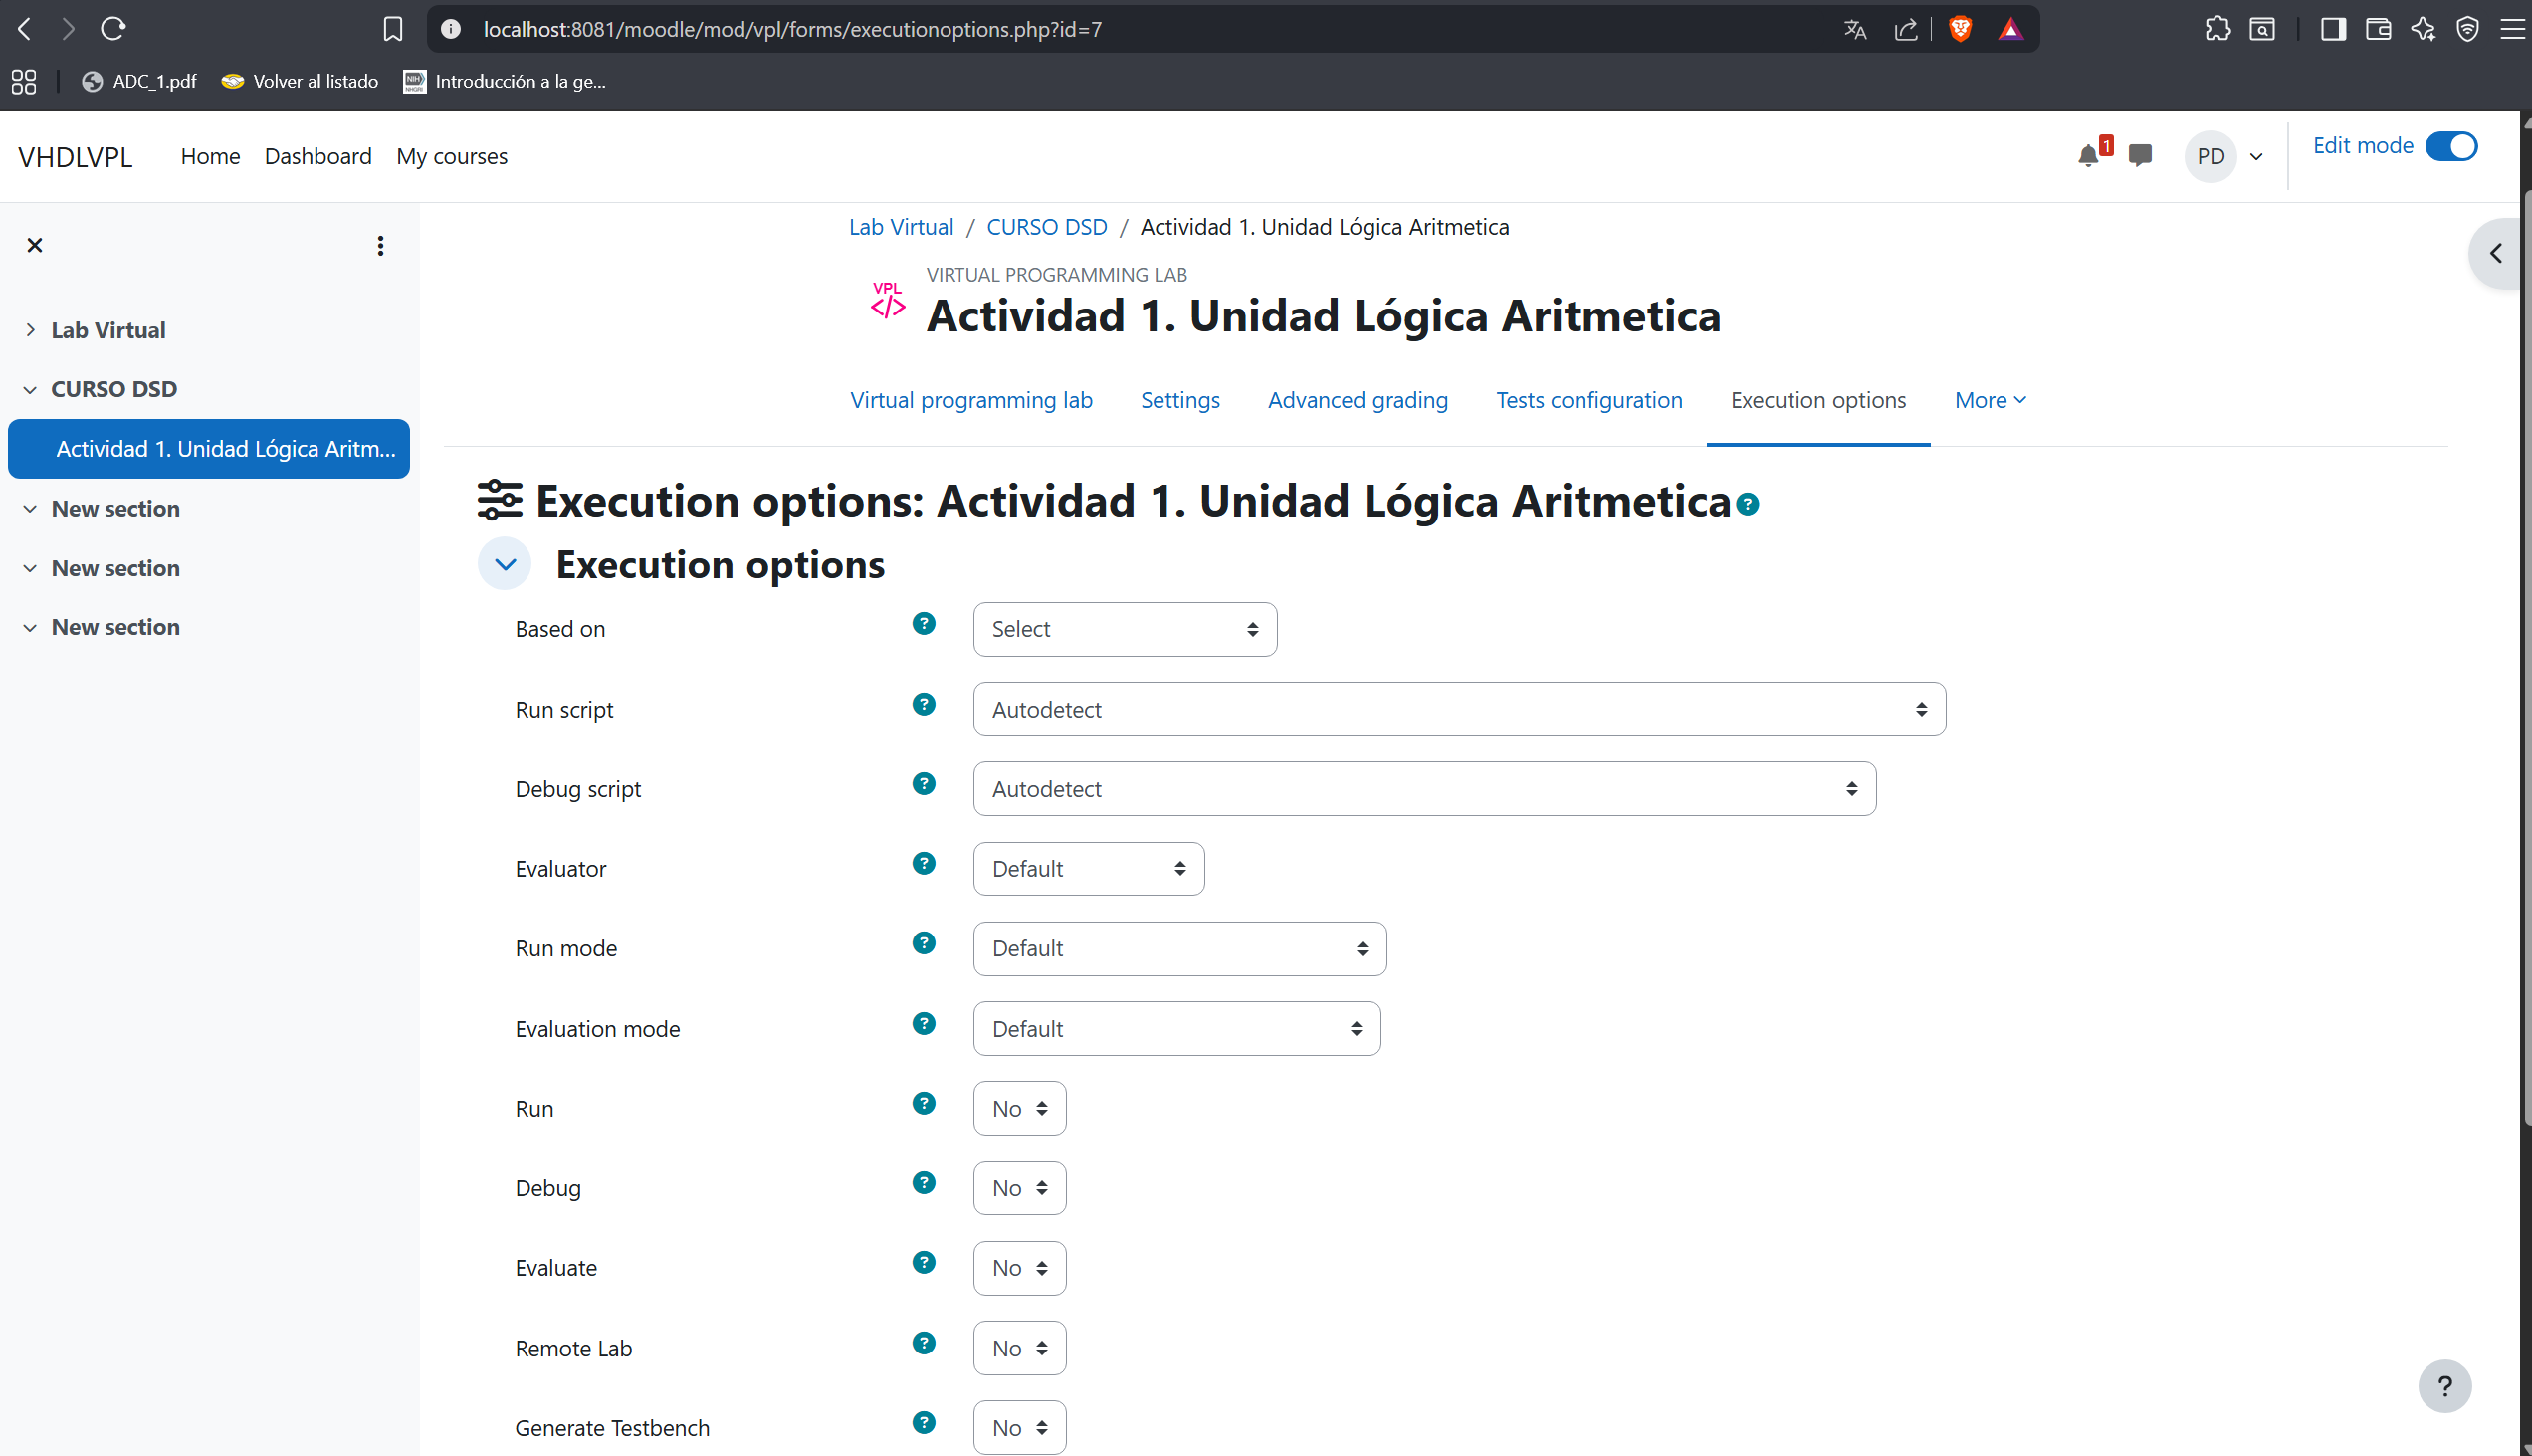
\includegraphics[width=1\textwidth]{profesor/opciones_ejecucion_vpl.png}
\caption{Opciones de ejecución en la actividad VPL}
\label{fig:opciones-ejecucion-vpl}
\end{figure} 

\begin{stepbox}{3}
  Dentro de esta sección lo mas importante es habilitar o deshabilitar las opciones de \textbf{Run} , \textbf{Debug} , \textbf{Remote Lab} , \textbf{Generate Testbench} y \textbf{Evaluate}, ya que estas son las acciones principales para que el alumno pueda ejecutar.
\end{stepbox}
\begin{figure}[H]
\centering
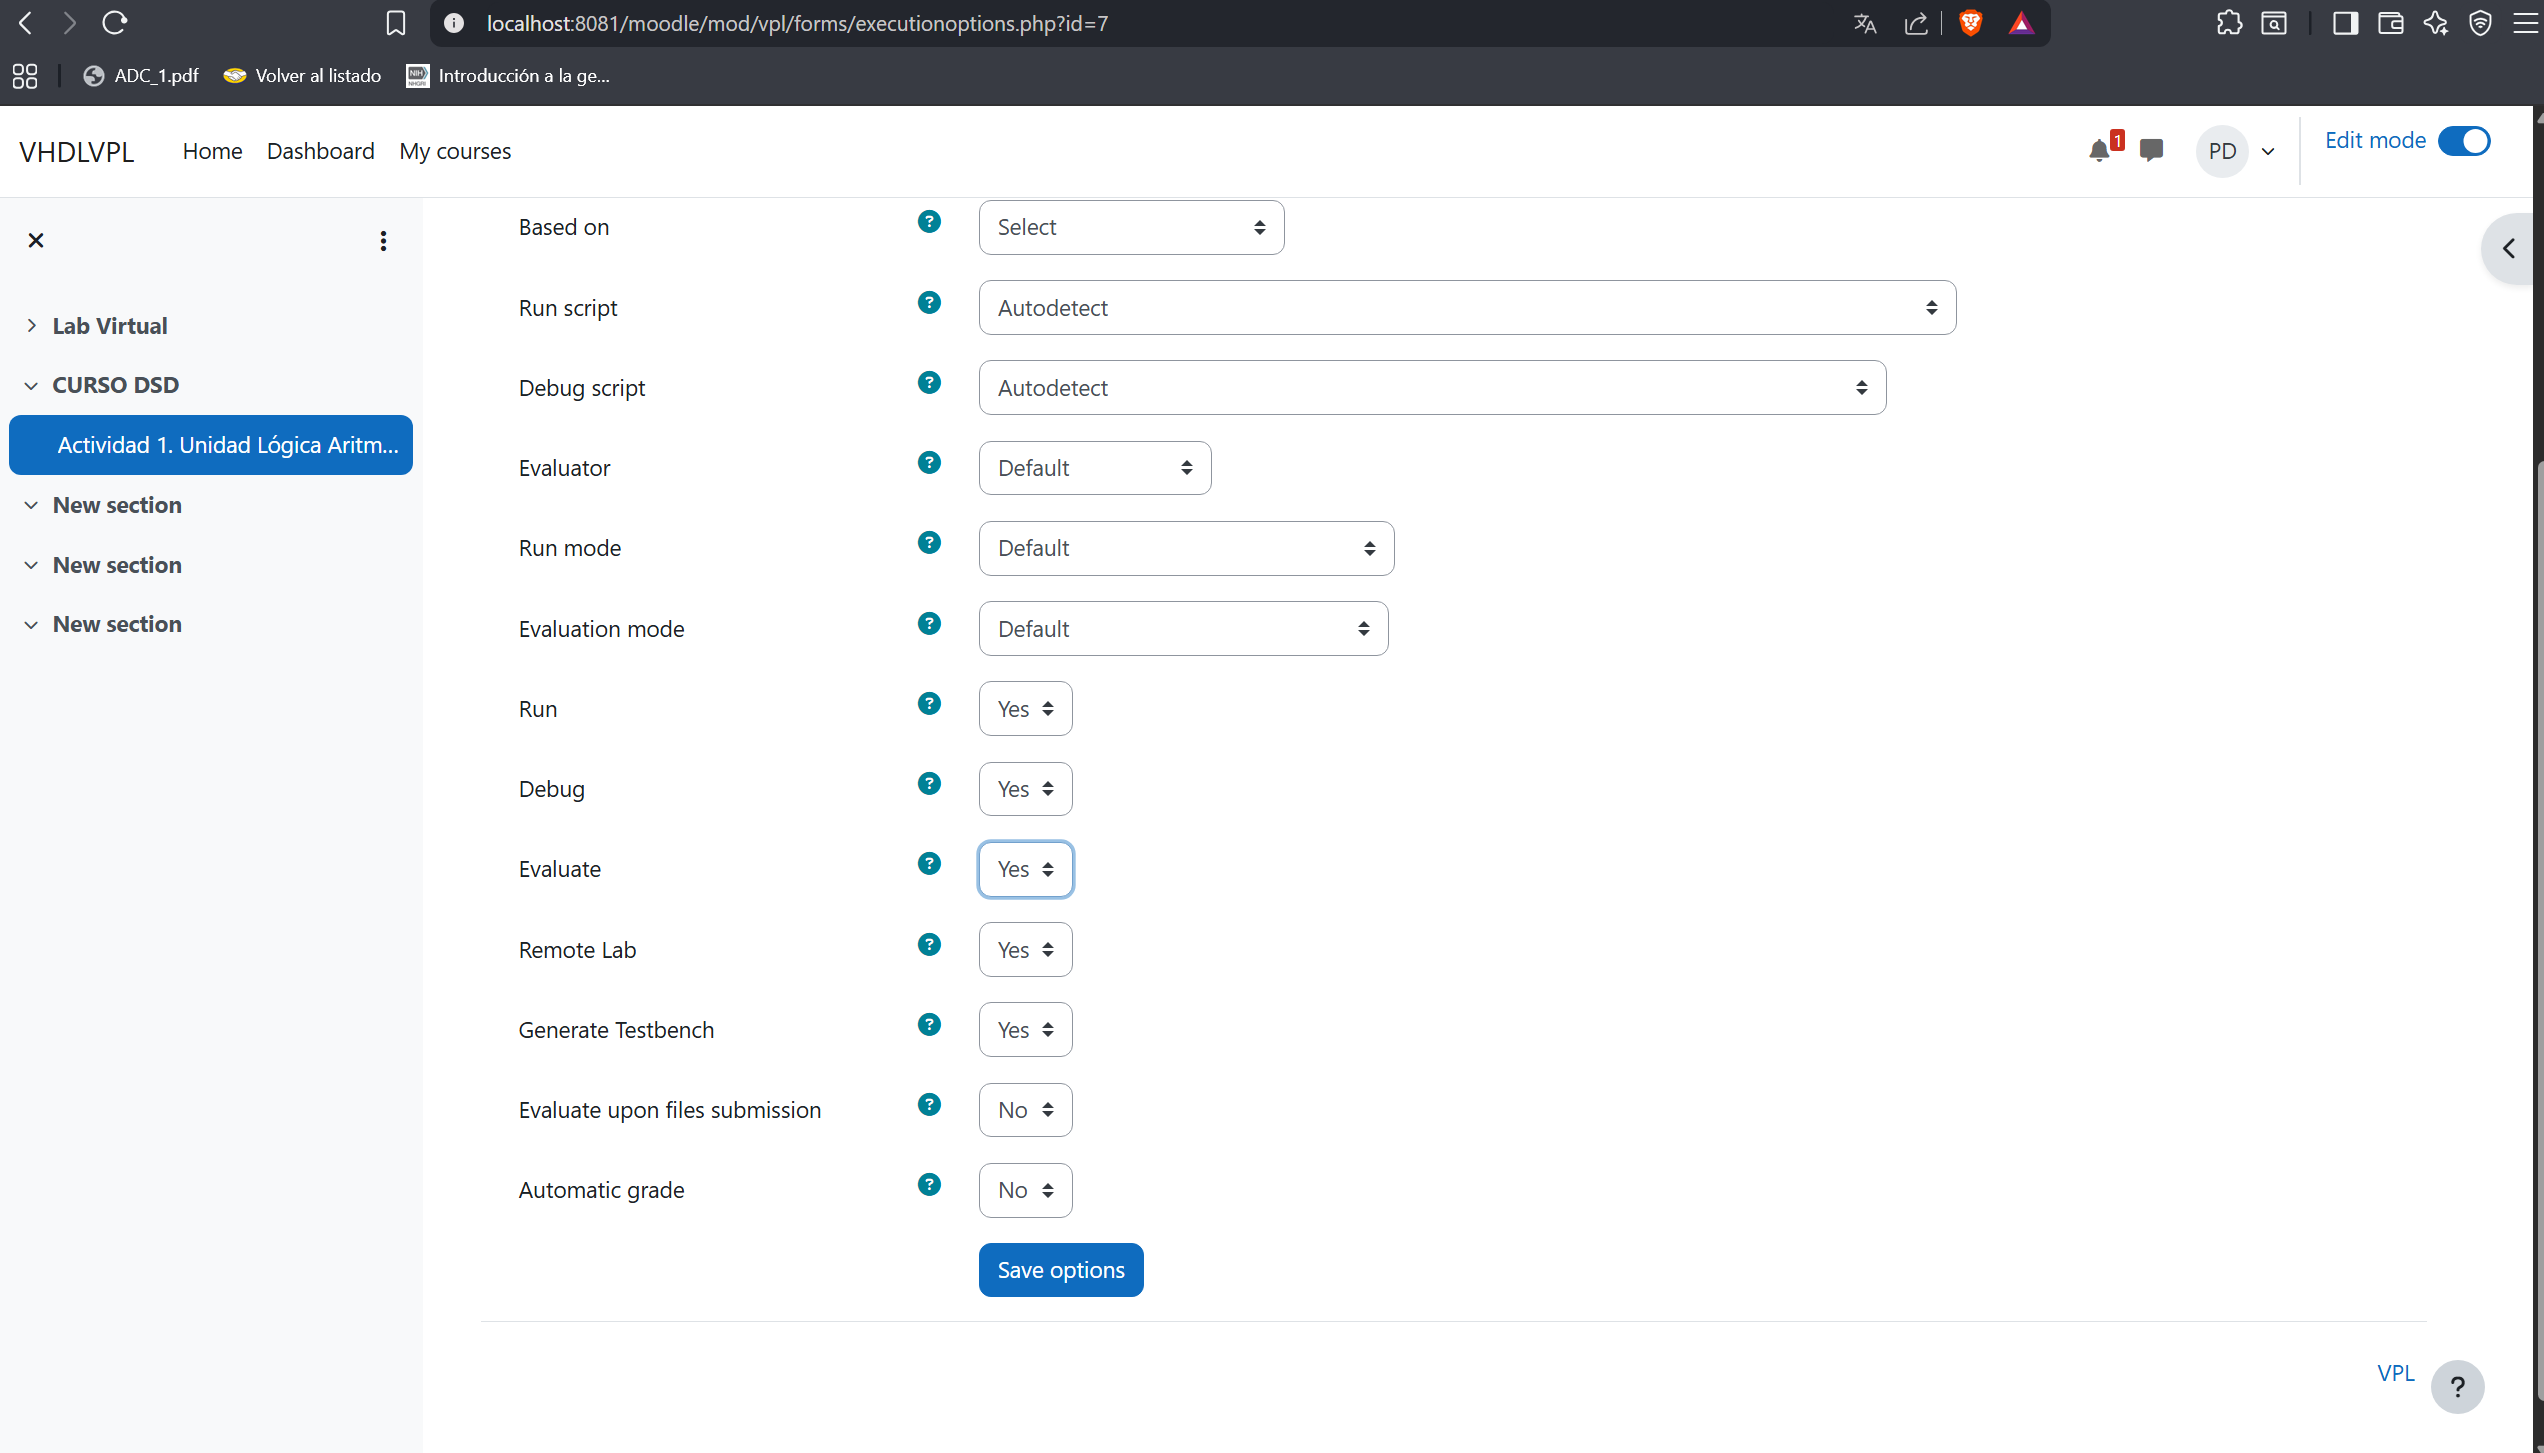
\includegraphics[width=1\textwidth]{profesor/permitir_opciones_vpl.png}
\caption{Permitir opciones de ejecución en la actividad VPL}
\label{fig:permitir_opciones}
\end{figure} 



% ── Capítulo 10 ─────────────────────────────────────────────
\chapter{Configuración de Casos de Prueba}
\label{ch:ficheros}

El archivo \archivo{vpl\_evaluate.cases} contiene los casos de prueba que el
evaluador \archivo{vpl\_evaluate.sh} ejecuta al calificar un diseño \vhdl.
El evaluador compila el código del alumno, detecta la entidad top, extrae sus
puertos, genera un testbench \vhdl automáticamente a partir de los casos, lo
simula con GHDL y calcula la nota final.

\section{Archivo \texttt{vpl\_evaluate.cases}}
\label{sec:vpl-evaluate-cases}

El archivo tiene dos bloques diferenciados:

\begin{enumerate}
  \item \textbf{Configuración global} --- parámetros que aplican a todos los
        casos (reloj, reset, tiempo de simulación). Aparecen antes del primer
        \texttt{case}.
  \item \textbf{Definición de casos} --- uno o más bloques \texttt{case}, cada
        uno con sus secciones \texttt{input:} y \texttt{output:}.
\end{enumerate}

Las líneas que comienzan con \texttt{\#} son comentarios y se ignoran.
Los nombres de parámetro son insensibles a mayúsculas y minúsculas.

\subsection{Sintaxis general de los casos de prueba}
\label{subsec:sintaxis-general}

\subsubsection{Configuración global}

Los parámetros globales se escriben como \texttt{parámetro = valor} y se
colocan al inicio del archivo, antes de cualquier \texttt{case}.
La Tabla~\ref{tab:params-global} lista los parámetros disponibles.

\begin{longtable}{L{3.6cm} L{3.2cm} L{5.7cm}}
  \caption{Parámetros de configuración global}
  \label{tab:params-global}\\
  \toprule
  \textbf{Parámetro} & \textbf{Ejemplo} & \textbf{Descripción} \\
  \midrule
  \endfirsthead
  \toprule
  \textbf{Parámetro} & \textbf{Ejemplo} & \textbf{Descripción} \\
  \midrule
  \endhead
  \bottomrule
  \endfoot
  \texttt{stop\_time\_all} & \texttt{1 ms} &
    Tiempo máximo de simulación global. \\
  \addlinespace
  \texttt{clock} & \texttt{CLK} &
    Nombre del puerto de reloj. Si se omite, el evaluador lo detecta
    automáticamente buscando puertos llamados \texttt{clk}, \texttt{clock}
    o \texttt{ck}. \\
  \addlinespace
  \texttt{clock\_period} & \texttt{10 ns} &
    Período completo del reloj. \\
  \addlinespace
  \texttt{reset} & \texttt{RESET} &
    Nombre del puerto de reset. Si se omite se busca entre
    \texttt{reset}, \texttt{rst}, \texttt{clr} y variantes con sufijo
    \texttt{\_n}. \\
  \addlinespace
  \texttt{reset\_active} & \texttt{1} &
    Nivel activo del reset: \texttt{1} = activo alto, \texttt{0} = activo
    bajo. \\
  \addlinespace
  \texttt{reset\_type} & \texttt{async} &
    Tipo de reset: \texttt{async} o \texttt{sync}. \\
  \addlinespace
  \texttt{reset\_cycles} & \texttt{2} &
    Ciclos de reloj durante los que se mantiene el reset al inicio de la
    simulación. \\
\end{longtable}

\subsubsection{Definición de un caso}

Cada caso comienza con la línea \texttt{case = \textit{descripción}} y contiene
los parámetros opcionales listados en la Tabla~\ref{tab:params-caso}, seguidos
de las secciones de señales.

\begin{longtable}{L{3.6cm} L{3.2cm} L{5.7cm}}
  \caption{Parámetros por caso de prueba}
  \label{tab:params-caso}\\
  \toprule
  \textbf{Parámetro} & \textbf{Ejemplo} & \textbf{Descripción} \\
  \midrule
  \endfirsthead
  \toprule
  \textbf{Parámetro} & \textbf{Ejemplo} & \textbf{Descripción} \\
  \midrule
  \endhead
  \bottomrule
  \endfoot
  \texttt{case} & \texttt{Prueba AND} &
    Nombre del caso; aparece en los reportes de fallo. \\
  \addlinespace
  \texttt{stop\_time} & \texttt{50 ns} &
    Tiempo de simulación específico para este caso.
    Sobreescribe \texttt{stop\_time\_all} solo para este caso. \\
  \addlinespace
  \texttt{grade reduction} & \texttt{25\%} &
    Penalización si el caso falla. Se admite porcentaje (\texttt{\%}) o
    valor absoluto. Si se omite, la penalización se reparte
    equitativamente entre todos los casos. \\
\end{longtable}

\subsubsection{Secciones de señales}

Dentro de cada caso se declaran dos secciones:

\begin{itemize}
  \item \texttt{input:} --- valores que se aplican a los puertos de entrada.
  \item \texttt{output:} --- valores esperados en los puertos de salida.
\end{itemize}

Cada señal se especifica en una línea indentada con el formato:

\begin{center}
  \texttt{~~~~NOMBRE\_SEÑAL = valor}
\end{center}

El valor puede ser:

\begin{itemize}
  \item \textbf{Escalar} --- un único vector de bits: \texttt{A = 1010}.
  \item \textbf{Array} --- varios valores para múltiples ciclos de reloj:
        \texttt{X = [0, 1, 1, 0]}.
  \item \textbf{Comodín} --- guion bajo \texttt{\_} dentro de un array de
        salida indica que ese ciclo no se verifica:
        \texttt{Z = [\_, \_, 1, 0]}.
\end{itemize}

Si alguna señal de entrada o salida usa sintaxis de array, el evaluador
activa el \textbf{modo secuencial}: genera un testbench que aplica un valor
por ciclo de reloj y verifica la salida al final de cada ciclo.
Sin arrays y sin reloj detectado, opera en \textbf{modo combinatorio}:
aplica las entradas, espera \texttt{stop\_time} y verifica las salidas una
sola vez.

\subsection{Sintaxis específica para evaluar código VHDL}
\label{subsec:sintaxis-vhdl}

\subsubsection{Circuitos combinatorios}

Para circuitos sin reloj se omite la configuración global de clock/reset.
El evaluador aplica los valores de \texttt{input:}, espera \texttt{stop\_time}
y compara las salidas declaradas en \texttt{output:}.

\begin{lstlisting}[caption={Caso combinatorio --- sumador de 4 bits con acarreo},
                   label={lst:cases-comb}]
# Tiempo de espera por defecto para todos los casos
stop_time_all = 50 ns

case = Suma basica sin acarreo
stop_time = 20 ns
grade reduction = 50%
input:
    A  = 0011
    B  = 0101
    Co = 0
output:
    S  = 1000
    C4 = 0

case = Suma con acarreo de entrada
stop_time = 20 ns
grade reduction = 50%
input:
    A  = 1111
    B  = 0001
    Co = 1
output:
    S  = 0001
    C4 = 1
\end{lstlisting}

\subsubsection{Circuitos secuenciales}

Para circuitos con reloj se declara la configuración global antes del primer
\texttt{case}. Los valores de entrada y salida se escriben como arrays
\texttt{[v0, v1, \ldots]}, donde cada elemento corresponde a un ciclo de
reloj. El evaluador genera el reloj, aplica el reset durante
\texttt{reset\_cycles} ciclos y luego recorre el array ciclo a ciclo.

\begin{lstlisting}[caption={Caso secuencial --- FSM Mealy},
                   label={lst:cases-seq}]
clock         = CLK
clock_period  = 10 ns
reset         = RESET
reset_active  = 0       # activo bajo
reset_type    = async
reset_cycles  = 2
stop_time_all = 1 ms

# Secuencia X=[0,0,1,1] desde estado inicial C
# Transiciones: C->B->A->B->C
case = Recorrido C-B-A-B-C
grade reduction = 60%
input:
    X = [0, 0, 1, 1]
output:
    Z1 = [1, 0, 1, 1]
    Z2 = [0, 1, 1, 0]

case = Una transicion C a B
grade reduction = 40%
input:
    X = [0]
output:
    Z1 = [1]
    Z2 = [0]
\end{lstlisting}

\begin{warnbox}[Longitud de arrays]
  Los arrays de \texttt{input:} y \texttt{output:} de un mismo caso deben
  tener la misma longitud. El evaluador no rellena valores faltantes.
\end{warnbox}

\subsubsection{Uso del comodín \texttt{\_}}

El comodín \texttt{\_} en un array de salida indica que ese ciclo no se
verifica. Es útil cuando la salida del circuito no está definida durante los
primeros ciclos (por ejemplo, mientras se llena un pipeline o un registro de
desplazamiento).

\begin{lstlisting}[caption={Comodin en salidas de registro de desplazamiento},
                   label={lst:cases-wildcard}]
clock         = CLK
clock_period  = 10 ns
reset         = CLR
reset_active  = 1
reset_type    = async
reset_cycles  = 2
stop_time_all = 1 ms

# Ciclo 1: carga L=1 -> Q=100000000000
# Ciclo 2: desplaza SHE=1 -> Q=010000000000
# Ciclo 3: desplaza SHE=1 -> Q=001000000000
case = Cargar y desplazar
grade reduction = 35%
input:
    L   = [1, 0, 0]
    SHE = [0, 1, 1]
    ES  = [0, 0, 0]
    D   = 100000000000
output:
    LED = [_, 0100010000000000, 0100001000000000]
\end{lstlisting}

% ── Capítulo 11 ─────────────────────────────────────────────
\chapter{Test de Evaluación por Parte del Profesor}
\label{ch:test-profesor}


% ── Apéndices ───────────────────────────────────────────────
\appendix

\chapter{Glosario de Términos}
\label{apx:glosario}
% VPL, VHDL, testbench, lógica reconfigurable, FPGA, etc.

\chapter{Referencia Rápida de Comandos}
\label{apx:referencia}
% Tabla de comandos GHDL, scripts de VPL

\chapter{Recursos y Referencias}
\label{apx:recursos}
% Documentación oficial VPL, IEEE VHDL, Moodle

% ── Bibliografía ────────────────────────────────────────────
\backmatter
\bibliographystyle{plain}
% \bibliography{referencias}

\end{document}
